\documentclass[12pt]{report}  
\usepackage{multirow}
\usepackage{makecell}
\usepackage{graphicx}
\usepackage{geometry}
\usepackage{amsmath}
\usepackage{amssymb}
\geometry{left=2.5cm,right=2.5cm,top=2.5cm,bottom=2.5cm}

\setcounter{secnumdepth}{3}
\begin{document}  
\title{\textbf{\LARGE Software Requirements Specification } \\ Volunteer Recruitment System \\ }

\author{ShuLan Tang 6516373\\\\WenChao Wang 6515783\\\\ ShangRong Cai 6515756\\\\ChengFeng Lao 6515766\\\\QiFei Chen 6515757 \\\\\\\\\\}    
\date{ November 16th 2016} 

 
\pagenumbering{gobble}
\maketitle
  \newpage

\tableofcontents
\newpage
 \pagenumbering{arabic}
\renewcommand\thesection{\arabic {section}}
\section{Introduction}

\subsection{Purpose}
\paragraph{}
The purpose of this document is to present a detailed description of the Volunteer Recruitment System. It will explain the purpose and features of the system, the interfaces of the system and what the system will do. This document is intended for both the stakeholders and the developers of the system.

\subsection{Scope of Project}
\paragraph{}
This software system will be a Web Publishing System for a volunteer recruitment. This system will be designed for managers to apply some activities for volunteers to take part in. By participating the volunteer activities, the system will give some integrals to users for applying a high identity.
More specifically, this system is designed to allow an manager to manage publish some socially useful activities and courses. Users can participate these activities. Beside, by participating these activities, more integrals will be got for applying a new identity. Different identities have different preferential policies for buying the courses which will be good for users.
\subsection{Introduction}
\paragraph{}
The system has two active actors, the user and the manager. Both of them are required to log in before they can access to the system, but only the user can sign up, which suppose the user to complete the personal information. 
The system can mainly be divided into three parts. First of all, the manager is able to initiate or edit projects that can be generated with QR code and courses, and then the user can enroll his/herself into the projects or the courses that should be paid and checked by the manager. Both of them have the access to view projects and courses lists. Besides, the user has the access to check and edit his/her personal information, as well as to check credit record, member manual, study record and activity record. Another function is that the user can submit application for his/her status. The last part is that the manager has the approach to searching users and viewing users list, users` details and user` credit records. In addition, the manager can also modify user records, identity authentication, edit discount strategy or charge information, as well as add activity records or charge information.

\subsection{Glossary}
\paragraph{}

\begin{tabular}{|c|l|}
\hline
Term & \makecell[c]{Definition} \\
\hline
User & A person who use the system to take part in activities. \\
\hline
Manager & A person who manage the system and in charge of the users.\\
\hline
\multirow{2}{*}{} 
Credit & \makecell[l]{Something can be gained after taking part in a activity and after \\ reaching a certain number can upgrade to a new status.} \\
\hline
\multirow{2}{*}{} 
Project & \makecell[l]{An offline activity that users can take part in, such as volunteering \\ work.} \\
\hline
\multirow{2}{*}{} 
Course & \makecell[l]{An offline activity that should pay money for, such as having lessons. }\\
\hline 
\multirow{2}{*}{} 
Status & \makecell[l]{A symbol as the user, some activities may decline users that not reach \\ a certain status, which can be upgrade when the credit is enough.} \\
\hline
Discount & Some courses have the discount that users can pay less. \\
\hline
\multirow{2}{*}{} 
Charge information & \makecell[l]{The information about bank that is used when the user remit for \\ joining a course.}\\
\hline
\end{tabular}

\subsection{Overview of Document}
\paragraph{}
The next chapter, the Overall Description section, of this document gives an overview of the functionality of the product. It describes the informal requirements and is used to establish a context for the technical requirements specification in the next chapter.
The third chapter, Requirements Specification section, of this document is written primarily for the developers and describes in technical terms the details of the functionality of the product. 
Both sections of the document describe the same software product in its entirety, but are intended for different audiences and thus use different language. And the last chapter is the database of this project which describes the database tables will be used.
\newpage
\section{Functional Requirements Specification}
\paragraph{}
This section outlines the use cases for each of the active readers separately. The manager and the users are main actors in this system.

\subsection{ User Use Case}
\subsubsection{Use case:  Check member manual}

\paragraph{}
Diagram: 
\begin{figure}[!htb]
  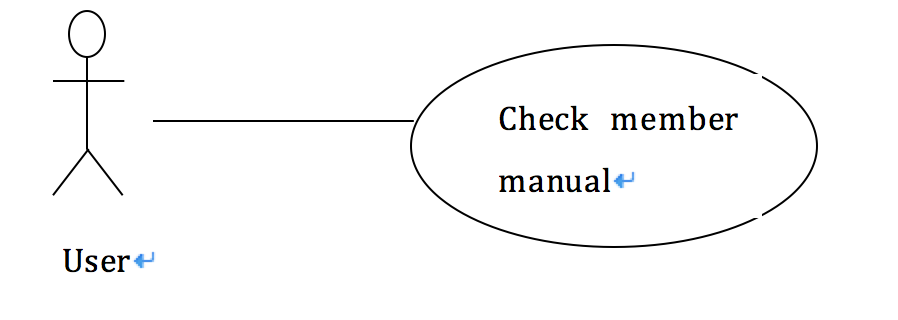
\includegraphics{1.PNG}
\end{figure}
\paragraph{}
\begin{flushleft}
\textbf{Brief Description }
\paragraph{}
The User access to his personal page and check his personal information. \\

\begin{flushleft}
\textbf{Initial Step-By-Step Description }
\paragraph{}
Before this use case can be built, the User has already registered and click on `personal information` at bottom right. 

\begin{flushleft}
1.	The system presents his personal information. \\
2.	The User can return to home page anytime. \\
Xref: Section 3.1.3, Check personal information
\end{flushleft}
\end{flushleft}
\end{flushleft}

\subsubsection{Use case:  Check credit record}
\newpage

\begin{figure}[!htb]
  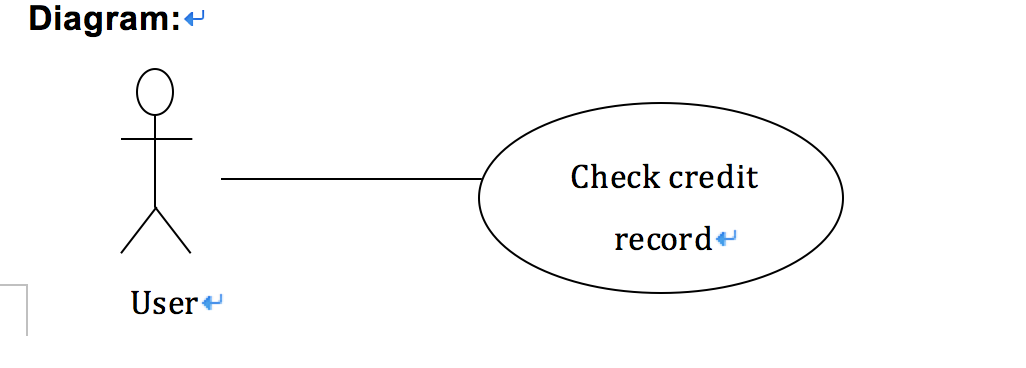
\includegraphics{2.PNG}
\end{figure}
\paragraph{}
\begin{flushleft}
\textbf{Brief Description }
\paragraph{}
The User access to his personal page, then check credit record. \\

\begin{flushleft}
\textbf{Initial Step-By-Step Description }
\paragraph{}
Before this use case can be built, the User has already registered and click on `personal information` at bottom right.

\begin{flushleft}
1.	The User selects to check credit record. \\
2.	The system presents his credit record every time. \\
3.	The User can return to his personal page anytime. \\
Xref: Section 3.1.2, Check credit record
\end{flushleft}
\end{flushleft}
\end{flushleft}

\subsubsection{Use case:  Check personal information }

\begin{figure}[!htb]
  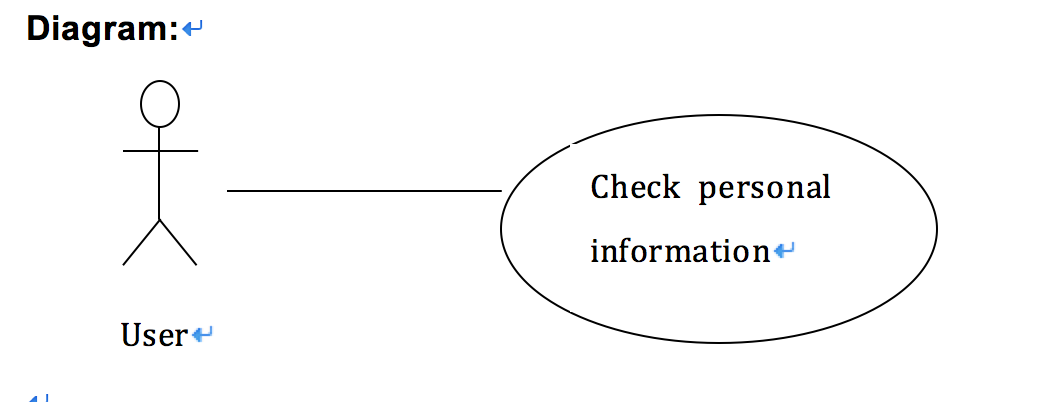
\includegraphics{3.PNG}
\end{figure}
\newpage
\paragraph{}
\begin{flushleft}
\textbf{Brief Description }
\paragraph{}
The User access to his personal page and check his personal information. \\

\begin{flushleft}
\textbf{Initial Step-By-Step Description }
\paragraph{}
Before this use case can be built, the User has already registered and click on `personal information` at bottom right.

\begin{flushleft}
1.	The system presents his personal information. \\
2.	The User can return to home page anytime. \\
Xref: Section 3.1.3, Check personal information.

\end{flushleft}
\end{flushleft}
\end{flushleft}

%4
\newpage
\subsubsection{Use case:  Check activity record  }

\begin{figure}[!htb]
  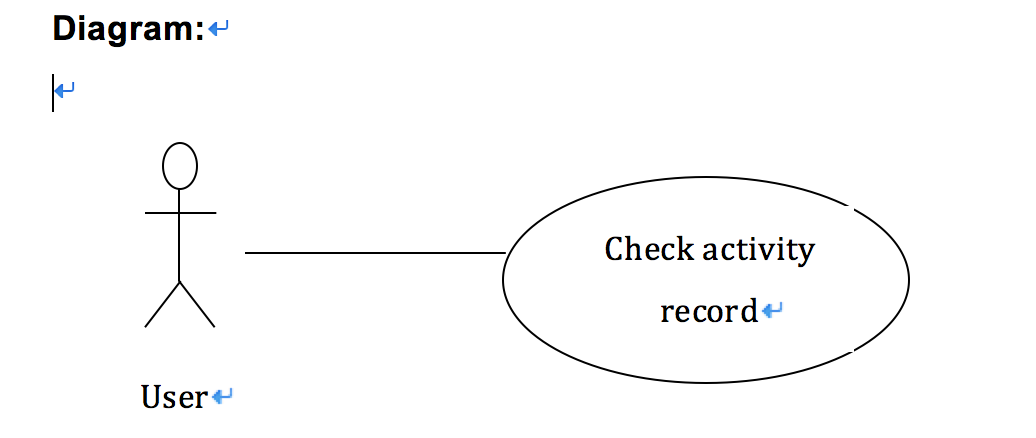
\includegraphics{4.PNG}
\end{figure}

\paragraph{}
\begin{flushleft}
\textbf{Brief Description }
\paragraph{}
The User access to his personal page and check his activity record. \\

\begin{flushleft}
\textbf{Initial Step-By-Step Description }
\paragraph{}
Before this use case can be built, the User has already registered and click on `personal information` at bottom right.

\begin{flushleft}
1.	The system shows his/her number of activity record. \\
2.	The User selects to `Activity record`. \\
3.	The system presents his activity record every time, and every record links to activity details. \\
4.	The User can return to his/her personal page anytime. \\
Xref: Section 3.1.4, Check activity record
\end{flushleft}
\end{flushleft}
\end{flushleft}



%5
\newpage
\subsubsection{Use case:  Submit application }

\begin{figure}[!htb]
  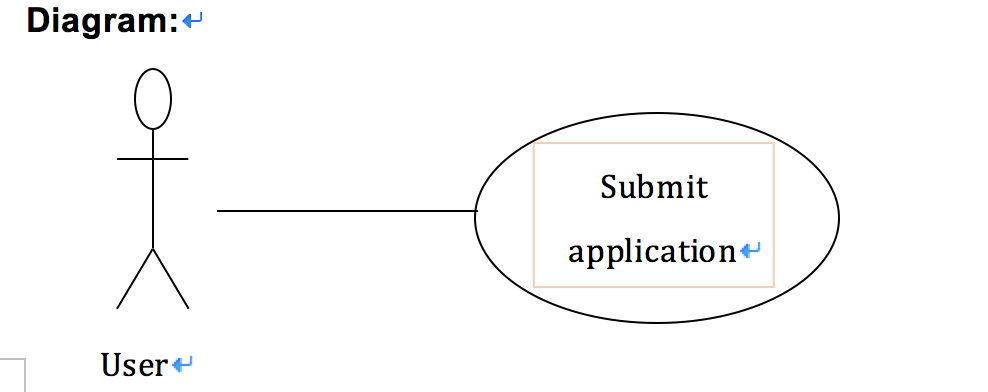
\includegraphics{5.PNG}
\end{figure}
\paragraph{}
\begin{flushleft}
\textbf{Brief Description }
\paragraph{}
If the User want to change his/her status, and he/she has enough credits, then he/she needs to submit his/her statement, and wait for manager review. \\

\begin{flushleft}
\textbf{Initial Step-By-Step Description }
\paragraph{}
Before this use case can be built, the User has already registered and click on `personal information` at bottom right.

\begin{flushleft}
1.	 The User selects the `status request`  button. \\
2.	The System shows a text area and a ?submit? button, and prompt User to write down his application. \\
3.	After finish, the User click `Submit`. \\
The System shows submit failed or succeeded, if failed, shows reason e.g. score were not enough, and show `Pending` at the previous ?Submit? button. \\
Xref: Section 3.1.5, Submit application
\end{flushleft}
\end{flushleft}
\end{flushleft}


%6
\newpage
\subsubsection{Use case:  Check study record}

\begin{figure}[!htb]
  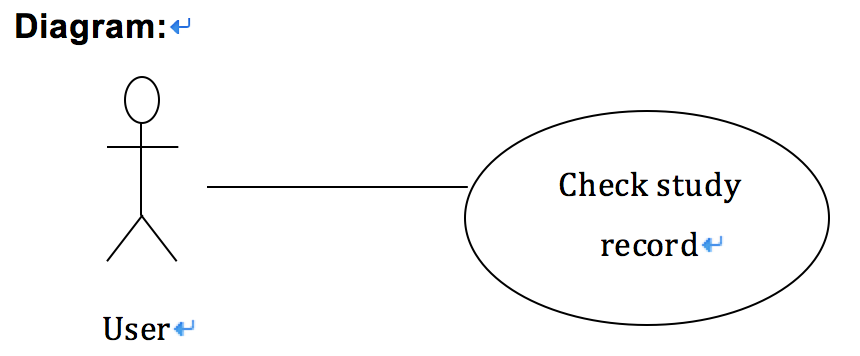
\includegraphics{6.PNG}
\end{figure}
\paragraph{}
\begin{flushleft}
\textbf{Brief Description }
\paragraph{}
The User access to his personal page and check his study record.\\

\begin{flushleft}
\textbf{Initial Step-By-Step Description }
\paragraph{}
Before this use case can be built, the User has already registered and click on `personal information` at bottom right.

\begin{flushleft}
1.	The system shows his/her number of activity record. \\
2.	The User selects to `Study record`. \\
3.	The system presents his/her study record every time, and every record links to details of the class. \\
4.	The User can return to his/her personal page anytime. \\
Xref: Section 3.1.6, Check study record.
\end{flushleft}
\end{flushleft}
\end{flushleft}


%7
\newpage
\subsubsection{Use case:  Attend projects }

\begin{figure}[!htb]
  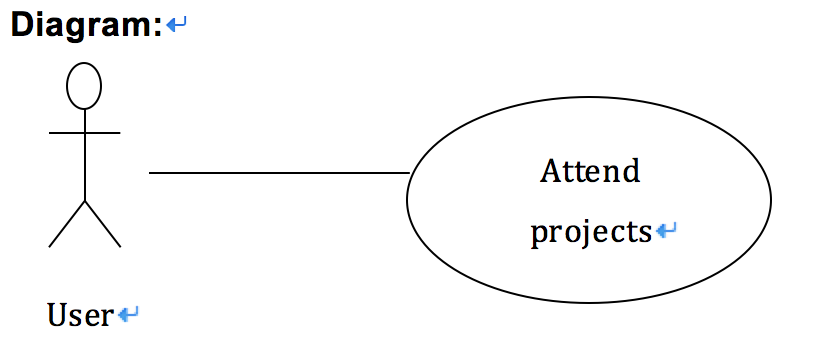
\includegraphics{7.PNG}
\end{figure}
\paragraph{}
\begin{flushleft}
\textbf{Brief Description }
\paragraph{}
The User logs in the WeChat Volunteering Website, attend projects.\\

\begin{flushleft}
\textbf{Initial Step-By-Step Description }
\paragraph{}
Before this use case can be initiated, the User has already logged in the WeChat Volunteering Website.

\begin{flushleft}
1.	The User chooses social activities. \\
2.	The System presents the list of projects information. \\
3.	The User chooses a project to attend. \\
4.	The System presents the details of the project. \\
5.	The User presses enroll button. \\
6.	The System enrolls the User in the database if the condition is satisfied. \\
Xref: Section 3.1.7, Attend projects
\end{flushleft}
\end{flushleft}
\end{flushleft}


%8
\newpage
\subsubsection{Use case:  View projects}

\begin{figure}[!htb]
  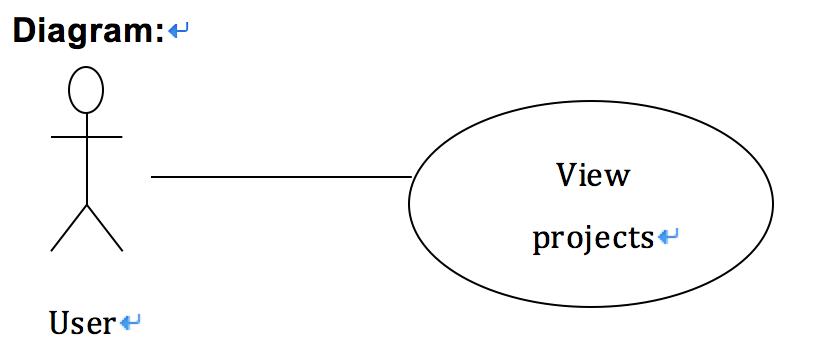
\includegraphics{8.PNG}
\end{figure}
\paragraph{}
\begin{flushleft}
\textbf{Brief Description }
\paragraph{}
The User logs in the WeChat Volunteering Website, view projects.\\

\begin{flushleft}
\textbf{Initial Step-By-Step Description }
\paragraph{}
Before this use case can be initiated, the User has already logged in the WeChat Volunteering Website.
\begin{flushleft}
1.	The User chooses social activities. \\
2.	The System presents the list of projects information. \\
3.	The User chooses a project.  \\
4.	The System presents the details of the project to the User. \\
Xref: Section 3.1.8, View projects

\end{flushleft}
\end{flushleft}
\end{flushleft}


%9
\newpage
\subsubsection{Use case: View Courses }

\begin{figure}[!htb]
  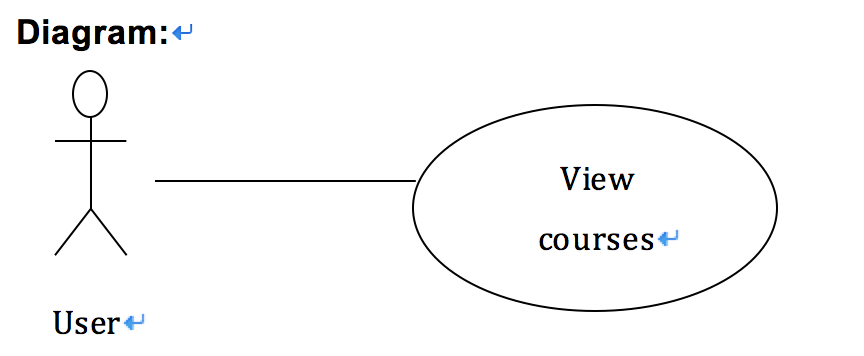
\includegraphics{9.PNG}
\end{figure}
\paragraph{}
\begin{flushleft}
\textbf{Brief Description }
\paragraph{}
The User logs in the WeChat Volunteering Website, view courses.\\

\begin{flushleft}
\textbf{Initial Step-By-Step Description }
\paragraph{}
Before this use case can be initiated, the User has already logged in the WeChat Volunteering Website .

\begin{flushleft}
1.	The User chooses course. \\
2.	The System presents the list of courses information. \\
3.	The User chooses a course. \\
4.	The System presents the details of the course to the User . \\
Xref: Section 3.1.9, View Courses

\end{flushleft}
\end{flushleft}
\end{flushleft}

%10
\newpage
\subsubsection{Use case:  Attend Course }

\begin{figure}[!htb]
  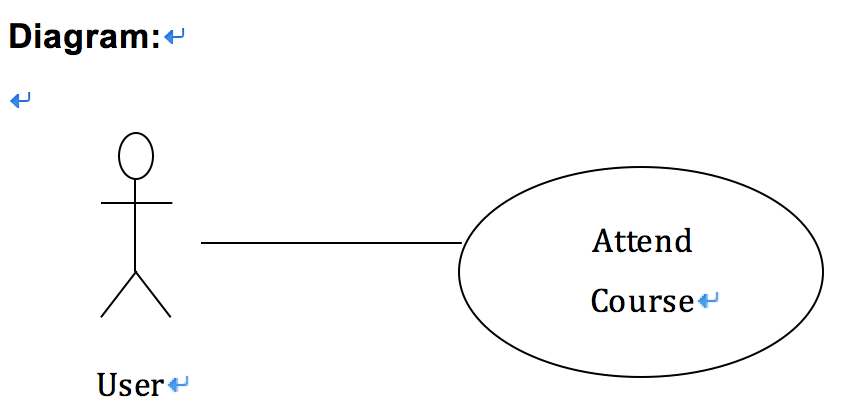
\includegraphics{10.PNG}
\end{figure}
\paragraph{}
\begin{flushleft}
\textbf{Brief Description }
\paragraph{}
The User logs in the WeChat Volunteering Website, attend projects.\\

\begin{flushleft}
\textbf{Initial Step-By-Step Description }
\paragraph{}
Before this use case can be initiated, the User has already logged in the WeChat Volunteering Website.
\begin{flushleft}
1.	The User chooses course. \\
2.	The system presents s list of courses. \\
3.	The User chooses a course to enroll. \\
4.	The system presents the details of the course. \\
5.	The User presses enroll button. \\
6.	The system presents a box containing a bank account and a button already paid. \\
7.	The User pays the course fee to the account and presses the button already paid. \\
Xref: Section 3.1.10, Attend Course

\end{flushleft}
\end{flushleft}
\end{flushleft}


%11
\newpage
\subsubsection{Use case:   Sign up }

\begin{figure}[!htb]
  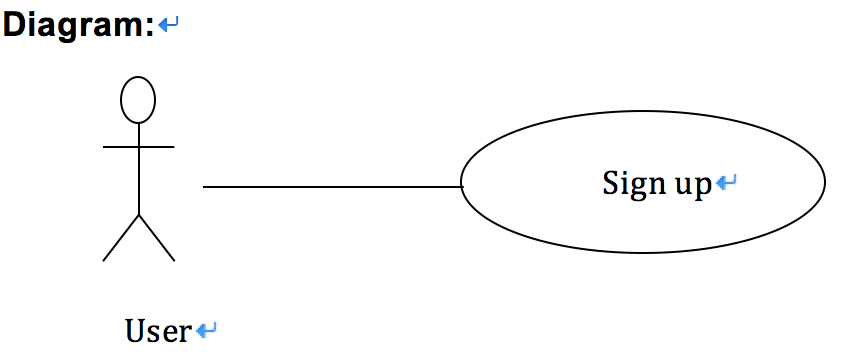
\includegraphics{11.PNG}
\end{figure}
\paragraph{}
\begin{flushleft}
\textbf{Brief Description }
\paragraph{}
The user access to the Wechat public number, go to the sign up page and complete the personal information.\\

\begin{flushleft}
\textbf{Initial Step-By-Step Description }
\paragraph{}
Before the user sign up, he/she needs to follow the Wechat public number with interest.

\begin{flushleft}
1.	The users choose to complete the member information. \\
2.	The system display the kinds of the information that the user need to fill. \\
3.	The users finish the information filling process. \\
The system records the user?s information and stores it to database. \\
Xref: Section 3.1.11, Sign up

\end{flushleft}
\end{flushleft}
\end{flushleft}


%12
\newpage
\subsubsection{Use case:  Log in }

\begin{figure}[!htb]
  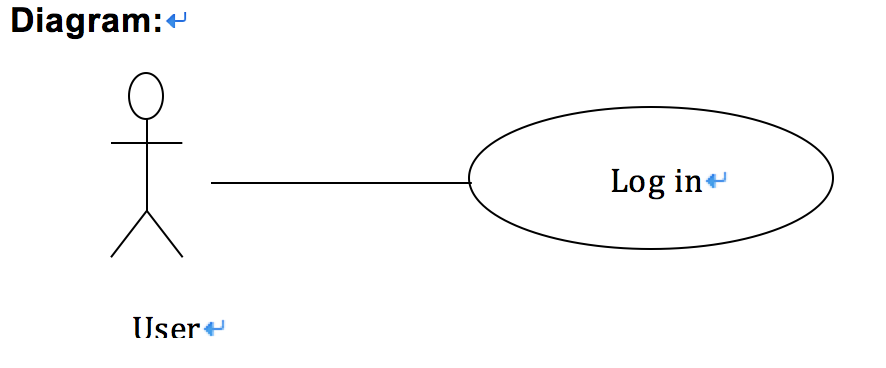
\includegraphics{12.PNG}
\end{figure}
\paragraph{}
\begin{flushleft}
\textbf{Brief Description }
\paragraph{}
The user goes to the log in page, enter the account and password, check the correctness and log into the system. \\

\begin{flushleft}
\textbf{Initial Step-By-Step Description }
\paragraph{}
Before the user sign up, he/she needs to sign up an account for logging in.

\begin{flushleft}
1.	The users choose to log into the system. \\
2.	The system displays the log in interface and asks the account and password. \\
3.	The users entering the account and password required for logging in. \\
4.	The system checks if the account and password are correct. \\
The user log into the system successfully or enter the account and password again. \\
Xref: Section 3.1.12, Log in

\end{flushleft}
\end{flushleft}
\end{flushleft}


%13
\newpage
\subsubsection{Use case:  Complete the personal information}
\paragraph{}
This use case is extended by the Sign up.
\begin{figure}[!htb]
  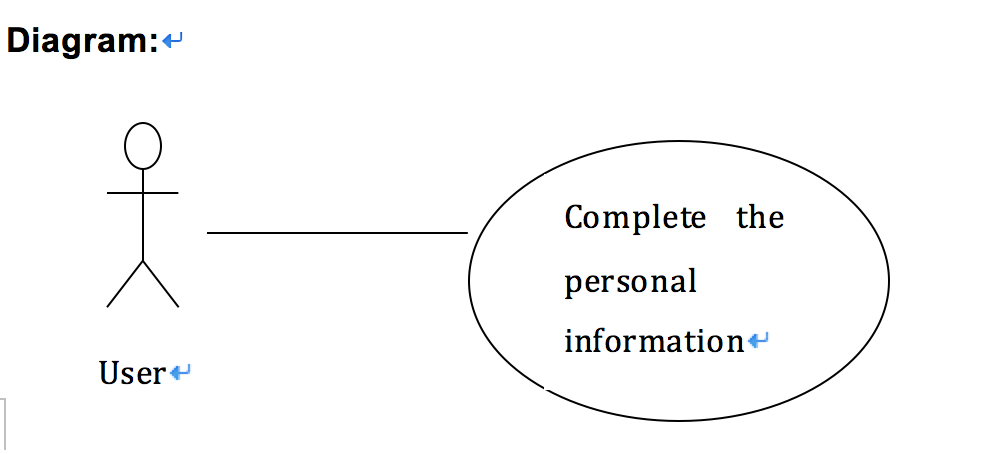
\includegraphics{13.PNG}
\end{figure}
\paragraph{}
\begin{flushleft}
\textbf{Brief Description }
\paragraph{}
When the user through the sign up process, he/she needs to complete the five different kinds of information which are name, telephone number, address, birthday and gender.\\

\begin{flushleft}
\textbf{Initial Step-By-Step Description }
\paragraph{}
Before the user completes the personal information, he/she needs to start the sign up process.

\begin{flushleft}
1.	The system provides the different kinds of information that want to be filled by user. \\
2.	The user tries to complete the five kinds of information. \\
3.	The system checks if the entering information format is correct. \\
4.	If the information is correct, the user signs up successfully, otherwise the user re-entering the member information. \\
Xref: Section 3.1.13, Complete the personal information 
\end{flushleft}
\end{flushleft}
\end{flushleft}

%14
\newpage
\subsubsection{Use case:  Edit the information }

\begin{figure}[!htb]
  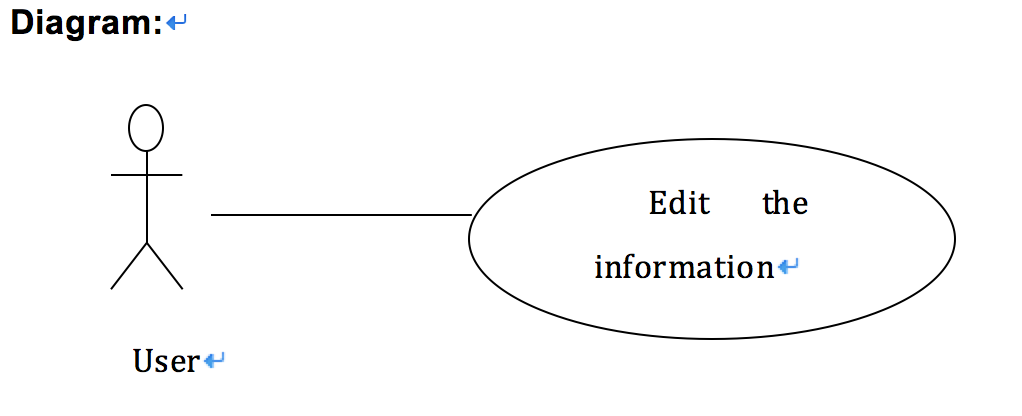
\includegraphics{14.PNG}
\end{figure}
\paragraph{}
\begin{flushleft}
\textbf{Brief Description }
\paragraph{}
The user goes to the personal information page, enters the change personal information and completes it.\\

\begin{flushleft}
\textbf{Initial Step-By-Step Description }
\paragraph{}
Before the user edit, he/she needs to access to the system.

\begin{flushleft}
1.	The user goes to the personal information page, click the edit link. \\
2.	The system presents the edit interface that the user can change the information. \\
3.	The user changed the information and save it. \\
4.	The system receives the information and save it to the database. \\
Xref: Section 3.1.14, Edit the information 
\end{flushleft}
\end{flushleft}
\end{flushleft}

%2.1
\newpage
\subsection{Manager Use Case} 
\subsubsection{Use case:  Initiate learning and growth}

\begin{figure}[!htb]
  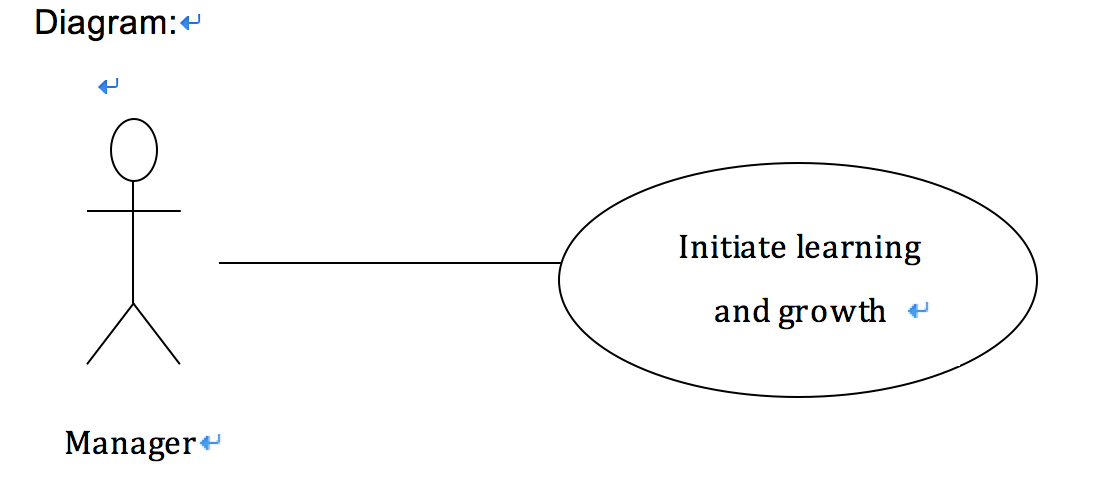
\includegraphics{21.PNG}
\end{figure}
\paragraph{}
\begin{flushleft}
\textbf{Brief Description }
\paragraph{}
The Manager accesses the Web to publish a new lesson which the users can look through some information about it and sign up for it. \\

\begin{flushleft}
\textbf{Initial Step-By-Step Description }
\paragraph{}
Before this use case can be initiated, the Manager has already accessed the Online Website.

\begin{flushleft}
1. The Manager selects to `Learning and Growth`. \\
2. The system displays the previous lessons has been initiated by Manager. \\
3. The Manager chooses `Add new` button. \\
4. The system displays the details which have to be filled by Manager. \\
5. The Manager fill in some details about this lesson including theme, start time, end time, address cost and so on. \\
6. The Manager press the `Publish` button. \\
7. The system transfers the lesson information to the website and returns the Manager to the main page of lesson. \\
Xref: Section 3.1.15, Initiate learning and growth


\end{flushleft}
\end{flushleft}
\end{flushleft}

%2.2
\newpage
\subsubsection{Use case:  Edit learning and growth}

\begin{figure}[!htb]
  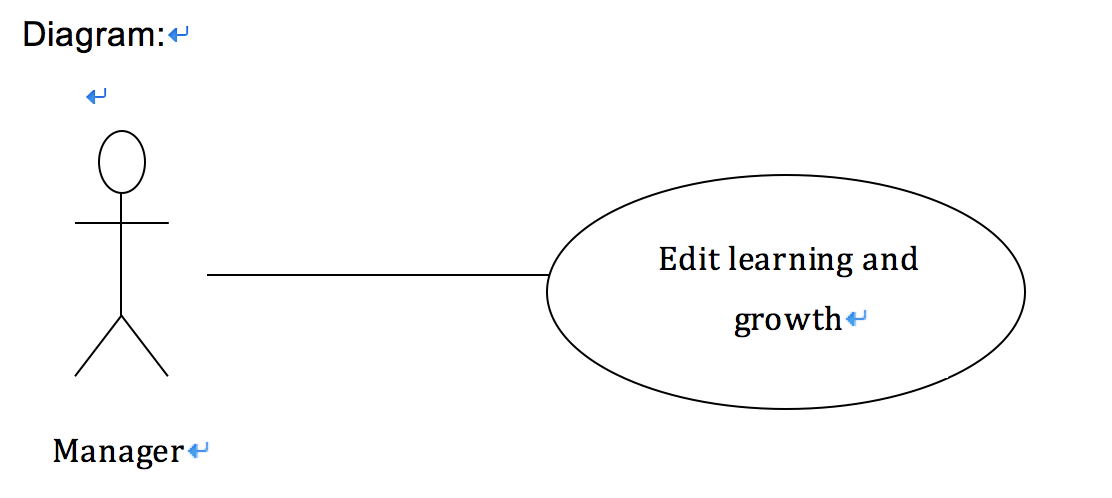
\includegraphics{22.PNG}
\end{figure}
\paragraph{}
\begin{flushleft}
\textbf{Brief Description }
\paragraph{}
The Manager accesses the Web to edit the `learning and growth` part.\\

\begin{flushleft}
\textbf{Initial Step-By-Step Description }
\paragraph{}
Before this use case can be initiated, the Manager has already accessed the Online Website.

\begin{flushleft}
1.	The Manager selects to `Learning and Growth. \\
2.	The system displays the previous lessons has been initiated by Manager. \\
3.	The Manager chooses one of the initiated lessons and press `Edit` button. \\
4.	The system displays the edit page. \\
5.	The Manager edits some details about this lesson and press the `Publish` button. \\
6.	The system transfers the lesson information to the website and returns the Manager to the main page of lesson. \\
Xref: Section 3.1.16, Edit learning and growth
\end{flushleft}
\end{flushleft}
\end{flushleft}


%2.3
\newpage
\subsubsection{Use case: Identity authentication}

\begin{figure}[!htb]
  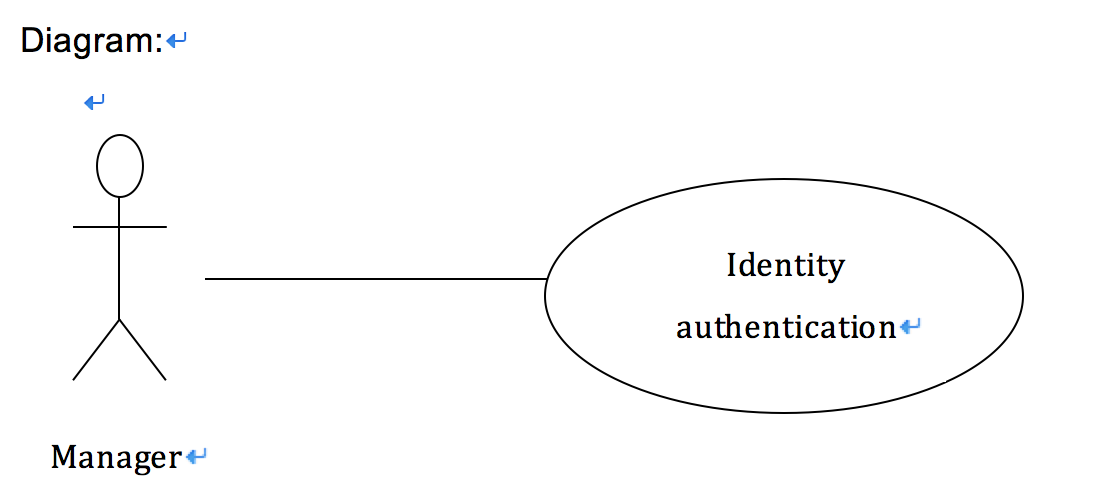
\includegraphics{23.PNG}
\end{figure}
\paragraph{}
\begin{flushleft}
\textbf{Brief Description }
\paragraph{}
The Manager accesses the Web to audit the users` status application and agree or disagree. \\

\begin{flushleft}
\textbf{Initial Step-By-Step Description }
\paragraph{}
Before this use case can be initiated, the Manager has already accessed the Online Website.

\begin{flushleft}
1.	The Manager selects to `Identity authentication`. \\
2.	The system displays the application list with applier names, identities, and apply time. \\
3.	The Manager can choose one of the applications. \\
4.	The system displays the detailed personal information and application statement. \\
5.	The Manager will choose `Agree` or `Disagree` based on the personal information.  \\
6.	The system will put this application into `Already Audited` page. \\
Xref: Section 3.1.17, Identity authentication
\end{flushleft}
\end{flushleft}
\end{flushleft}


%2.4
\newpage
\subsubsection{Use case:  Add activity records }

\begin{figure}[!htb]
  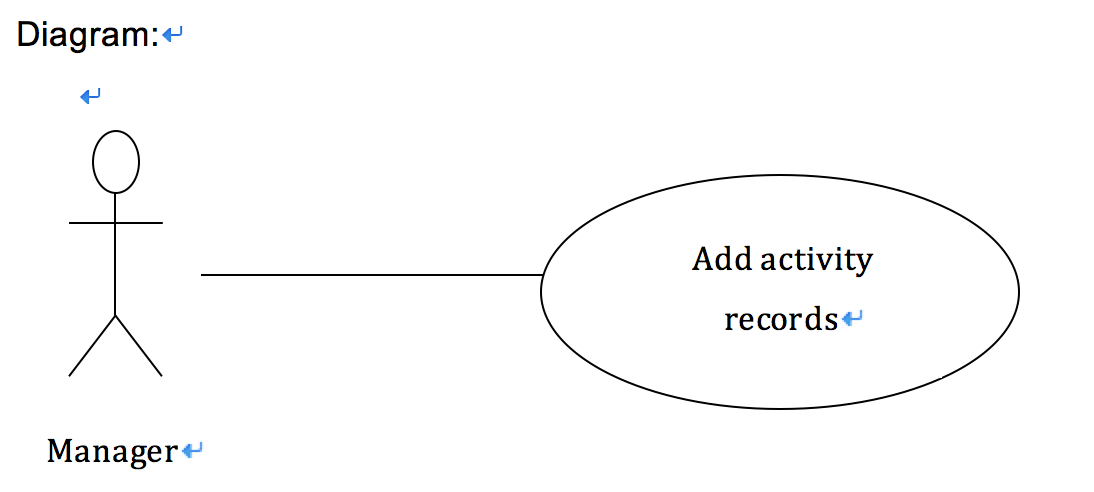
\includegraphics{24.PNG}
\end{figure}
\paragraph{}
\begin{flushleft}
\textbf{Brief Description }
\paragraph{}
The Manager accesses the Web to add activity records which describe the details of the activity that has just been completed and all of the users can look through them.\\

\begin{flushleft}
\textbf{Initial Step-By-Step Description }
\paragraph{}
Before this use case can be initiated, the Manager has already accessed the Online Website.

\begin{flushleft}
1.	The Manager selects to `Activity records`. \\
2.	The system displays the previous activity records. \\
3.	The Manager chooses `Add new` button. \\
4.	The system displays some details which Manager have to fill in. \\
5.	The Manager fills in the details and publish the records. \\
6.	The system transfers records to the website and returns Manager to the main page. \\
Xref: Section 3.1.18, Add activity records
\end{flushleft}
\end{flushleft}
\end{flushleft}


%2.5
\newpage
\subsubsection{Use case:  View users list }

\begin{figure}[!htb]
  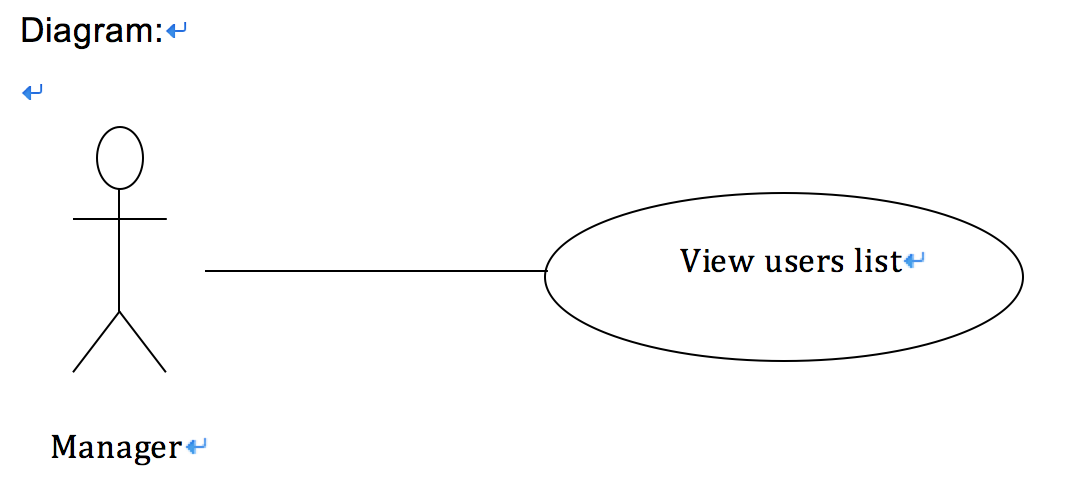
\includegraphics{25.PNG}
\end{figure}
\paragraph{}
\begin{flushleft}
\textbf{Brief Description }
\paragraph{}
The Manager accesses the Web to view users list which have sign up to the website.\\

\begin{flushleft}
\textbf{Initial Step-By-Step Description }
\paragraph{}
Before this use case can be initiated, the Manager has already accessed the Online Website.

\begin{flushleft}
1.	The Manager selects to `View users`. \\
2.	The system displays the users list including users` basic information. \\
Xref: Section 3.1.19, View users list
\end{flushleft}
\end{flushleft}
\end{flushleft}

%2.6
\newpage
\subsubsection{Use case:  Search users }

\begin{figure}[!htb]
  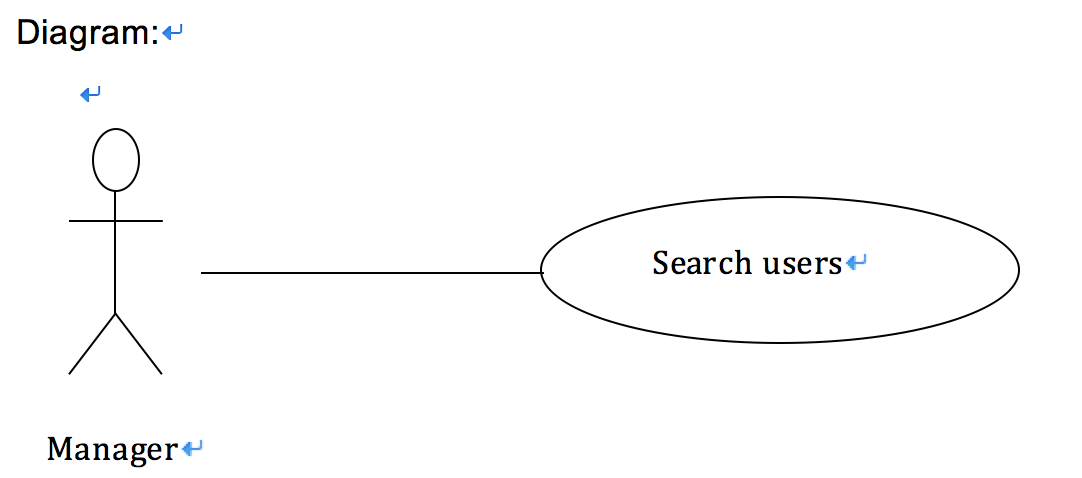
\includegraphics{26.PNG}
\end{figure}
\paragraph{}
\begin{flushleft}
\textbf{Brief Description }
\paragraph{}
The Manager accesses the Web to publish a new lesson which the users can look through some information about it and sign up for it.\\

\begin{flushleft}
\textbf{Initial Step-By-Step Description }
\paragraph{}
Before this use case can be initiated, the Manager has already accessed the Online Website.

\begin{flushleft}
1.	The Manager selects to `Search users`. \\
2.	The system displays the window of the search. \\
3.	The Manager type user`s phone number that want to search. \\
4.	The system displays user information whose phone number is searched. \\
Xref: Section 3.1.20, Search users
\end{flushleft}
\end{flushleft}
\end{flushleft}

%2.7
\newpage
\subsubsection{Use case:  View users?`details }

\begin{figure}[!htb]
  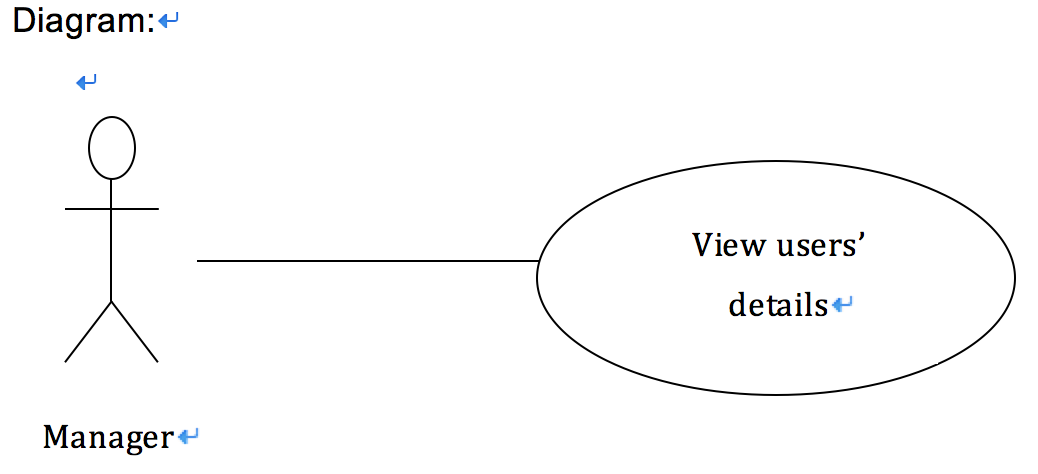
\includegraphics{27.PNG}
\end{figure}
\paragraph{}
\begin{flushleft}
\textbf{Brief Description }
\paragraph{}
The Manager accesses the Web to view the detailed information of users.\\

\begin{flushleft}
\textbf{Initial Step-By-Step Description }
\paragraph{}
Before this use case can be initiated, the Manager has already accessed the Online Website.

\begin{flushleft}
1.	The Manager selects to `View users`. \\
2.	The system displays the users list. \\
3.	The Manager can choose one specific user. \\
4.	The system displays the detailed personal information of the user. \\
Xref: Section 3.1.21, View users? details
\end{flushleft}
\end{flushleft}
\end{flushleft}

%2.8
\newpage
\subsubsection{Use case:  Generate QR Code }

\begin{figure}[!htb]
  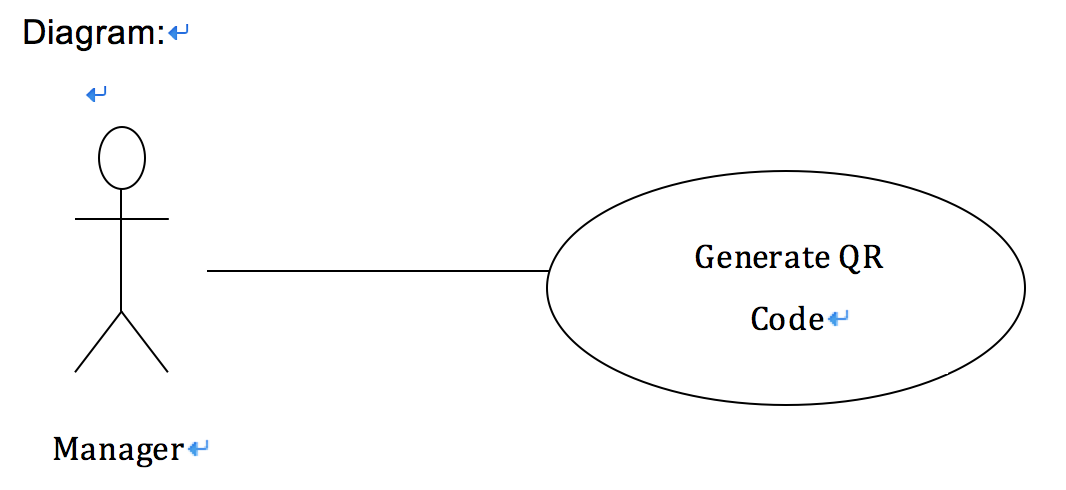
\includegraphics{28.PNG}
\end{figure}
\paragraph{}
\begin{flushleft}
\textbf{Brief Description }
\paragraph{}
The Manager generate QR code before activities start to make volunteers to scan it which can be used as attendance sheet.\\

\begin{flushleft}
\textbf{Initial Step-By-Step Description }
\paragraph{}
Before this use case can be initiated, the Manager has already accessed the Online Website.

\begin{flushleft}
1.	The Manager selects to `View activities`. \\
2.	The system displays the public-spirited activities which are not be held. \\
3.	The Manager can choose `Generate QR code` button.  \\
4.	The system generates the QR code and displays it on the screen.  \\
Xref: Section 3.1.22, Generate QR Code
\end{flushleft}
\end{flushleft}
\end{flushleft}

%2.9
\newpage
\subsubsection{Use case:  Modify user credit}

\begin{figure}[!htb]
  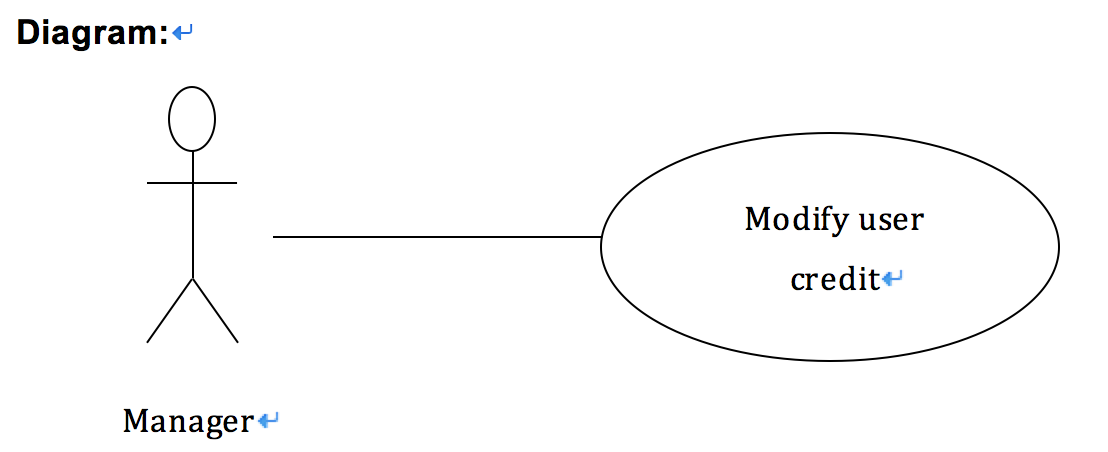
\includegraphics{29.PNG}
\end{figure}
\paragraph{}
\begin{flushleft}
\textbf{Brief Description }
\paragraph{}
The Manager accesses the management system, searches for a user using phone number and modify his/her credit.\\

\begin{flushleft}
\textbf{Initial Step-By-Step Description }
\paragraph{}
Before this use case can be initiated, the Manager has already accessed the manager interface and select Credit Management section.

\begin{flushleft}
1.	The manager types in user`s phone number. \\
2.	The system displays the user`s name. \\
3.	The manager types in number of credits want to modify. \\
4.	The manager chooses the reason of modification among charity activity, courses and other. \\
5.	The manager confirms modification. \\
6.	The system modify user credit record.  \\
Xref: Section 3.1.23, Modify user credit
\end{flushleft}
\end{flushleft}
\end{flushleft}

%2.10
\newpage
\subsubsection{Use case:  View users` credit records }

\begin{figure}[!htb]
  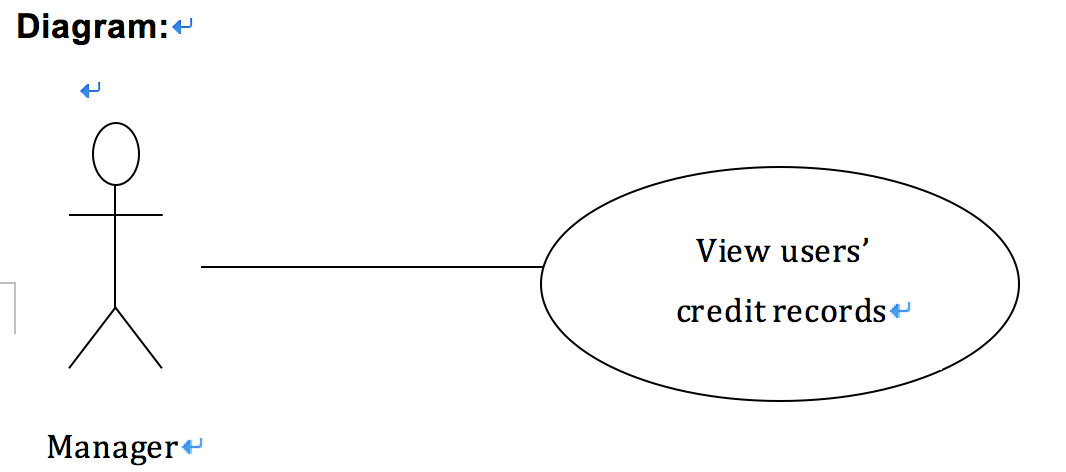
\includegraphics{210.PNG}
\end{figure}
\paragraph{}
\begin{flushleft}
\textbf{Brief Description }
\paragraph{}
The manager view a list of record of all credit modification. \\

\begin{flushleft}
\textbf{Initial Step-By-Step Description }
\paragraph{}
Before this use case can be initiated, the Manager has already accessed the manager interface.

\begin{flushleft}
1.	The Manager chooses the credit management button.  \\
2.	The System shows the list of all credit modification record, sorted by time. \\
3.	The Manager clicks one user`s name. \\
4.	The System displays this user`s credit modification records. \\
Xref: Section 3.1.24, View users? credit records
\end{flushleft}
\end{flushleft}
\end{flushleft}

%2.11
\newpage
\subsubsection{Use case:  Add charge information }

\begin{figure}[!htb]
  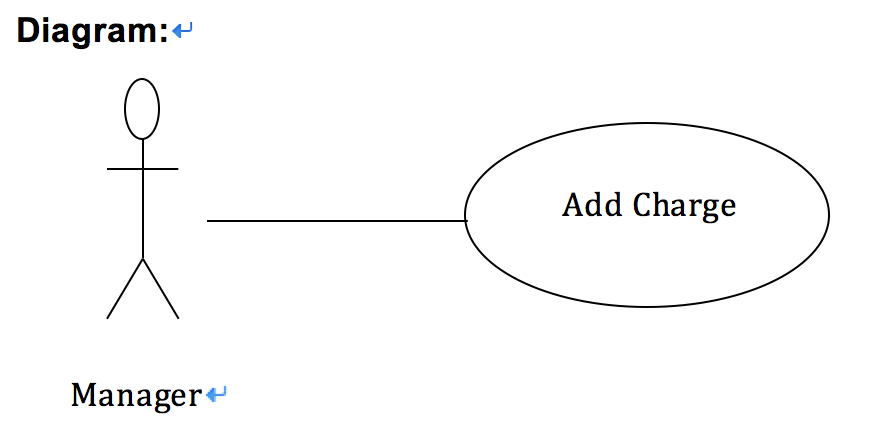
\includegraphics{211.PNG}
\end{figure}
\paragraph{}
\begin{flushleft}
\textbf{Brief Description }
\paragraph{}
The Manager add a charge information into system. \\

\begin{flushleft}
\textbf{Initial Step-By-Step Description }
\paragraph{}
Before this use case can be initiated, the Manager has already accessed the manager interface.

\begin{flushleft}
1.	The Manager chooses Finance Management button. \\
2.	The System display current accounts information. \\
3.	The Manager clicks New Account button. \\
4.	The System prompts Manager types in Name, Bank Name, and Account number. \\
5.	The Manager types in information. \\
6.	The Manager clicks Save button. \\
7.	The new account information saved in the system. \\
Xref: Section 3.1.25, Add charge information
\end{flushleft}
\end{flushleft}
\end{flushleft}

%2.12
\newpage
\subsubsection{Use case:  Update Charge information }

\begin{figure}[!htb]
  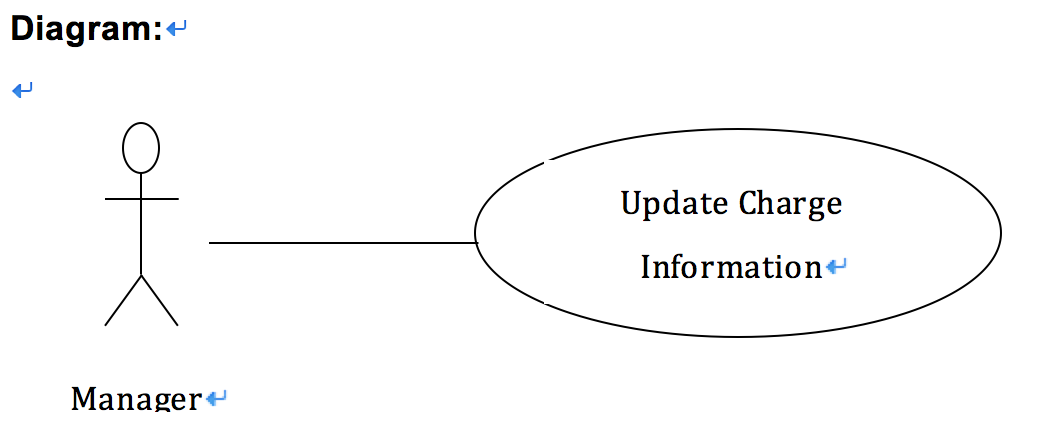
\includegraphics{212.PNG}
\end{figure}
\paragraph{}
\begin{flushleft}
\textbf{Brief Description }
\paragraph{}
The Manager edit a charge information in system. \\

\begin{flushleft}
\textbf{Initial Step-By-Step Description }
\paragraph{}
Before this use case can be initiated, the Manager has already accessed the manager interface.

\begin{flushleft}
1.	The Manager chooses Finance Management button.  \\
2.	The System displays a list current account information. \\
3.	The Manager chooses a current account information and clicks on Edit button. \\
4.	The system presents an input area filling in with the information. \\
5.	The Manager modifies the information and submits the form. \\
6.	The system verifies the information and returns the Manager to current account list page. \\
Xref: Section 3.1.26, Update Charge information

\end{flushleft}
\end{flushleft}
\end{flushleft}

%2.13
\newpage
\subsubsection{Use case:  Edit Discount Strategy }

\begin{figure}[!htb]
  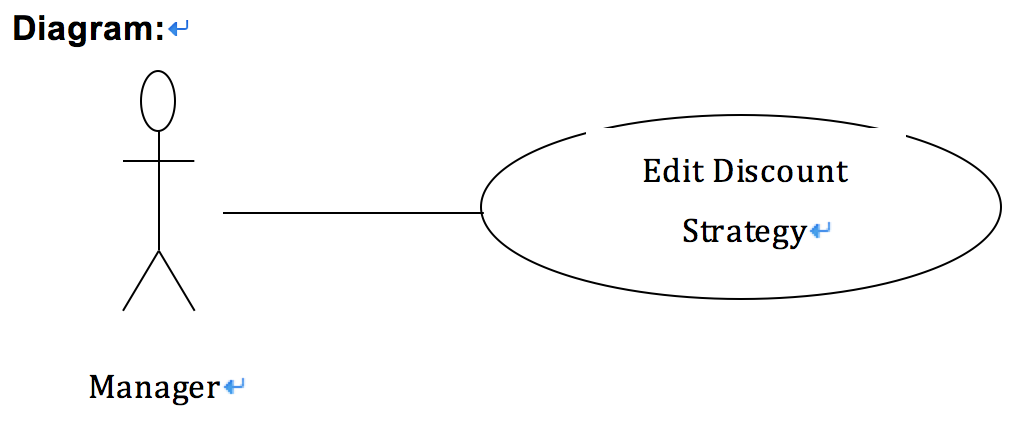
\includegraphics{213.PNG}
\end{figure}
\paragraph{}
\begin{flushleft}
\textbf{Brief Description }
\paragraph{}
The Manager add a discount strategy of courses into system. \\

\begin{flushleft}
\textbf{Initial Step-By-Step Description }
\paragraph{}
Before this use case can be initiated, the Manager has already accessed the manager interface.

\begin{flushleft}
1.	The Manager chooses Discount Management button. \\
2.	The System displays current discount information with five different discount number for users with different number of credits, before the first initialization, all numbers are zero. \\
3.	The Manager clicks edit button. \\
4.	The System enable Manager modify five numbers(percentage). \\
5.	The Manager modifies five discount numbers and clicks Save button. \\
6.	The system verifies the information and returns the Manager to Discount Management page. \\
Xref: Section 3.1.27, Edit Discount Strategy
\end{flushleft}
\end{flushleft}
\end{flushleft}

%2.14
\newpage
\subsubsection{Use case:  Initial projects }

\begin{figure}[!htb]
  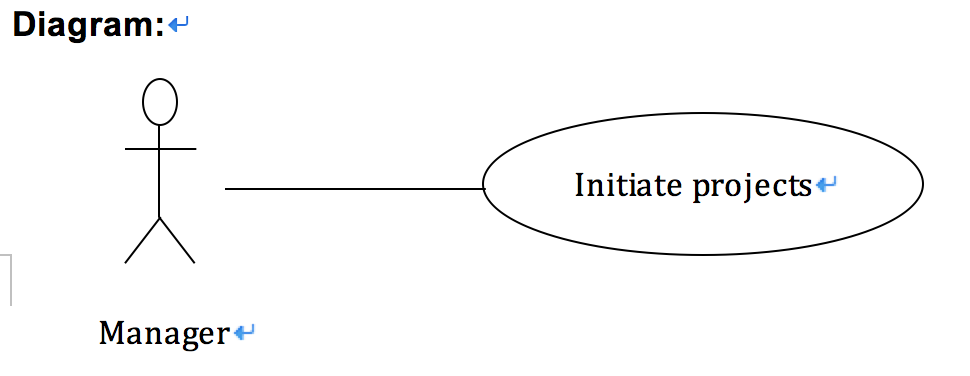
\includegraphics{214.PNG}
\end{figure}
\paragraph{}
\begin{flushleft}
\textbf{Brief Description }
\paragraph{}
The Manager logs in the WeChat Volunteering Website, releases the project so that Users can take part in. \\

\begin{flushleft}
\textbf{Initial Step-By-Step Description }
\paragraph{}
Before this use case can be initiated, the Manager has already logged in the WeChat Volunteering Website.

\begin{flushleft}
1.	The Manager chooses social activities. \\
2.	The system presents the list of projects that have finished. \\
3.	The Manager presses add project record. \\
4.	The system shows a new page with empty project information to be completed. \\
5.	The Manager complete the subject, start time, end time, detailed address of the project, the number of volunteers limited, score and identity needed, as well as award. \\
6.	The Manager presses the text area for describing project details. \\
7.	The system presents an input box for typing to the Administer. \\
8.	The Manager presses finish to submit project details including photos and videos. \\
9.	The system returns to the previous page.\\
10.	The Manager presses preview button. \\
11.	The system shows the appearance of the project after submitted. \\
12.	The Manager presses release button. \\
13.	The system releases the project so that Users can take part in. \\
Xref: Section 3.1.28, Initial projects

\end{flushleft}
\end{flushleft}
\end{flushleft}

%2.15
\newpage
\subsubsection{Use case:  Edit projects }

\begin{figure}[!htb]
  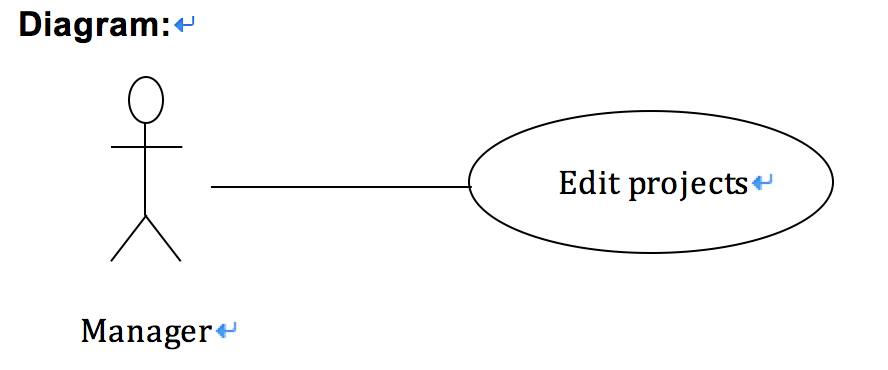
\includegraphics{215.PNG}
\end{figure}
\paragraph{}
\begin{flushleft}
\textbf{Brief Description }
\paragraph{}
The Manager logs in the WeChat Volunteering Website, edit projects.\\

\begin{flushleft}
\textbf{Initial Step-By-Step Description }
\paragraph{}
Before this use case can be initiated, the Manager has already logged in the WeChat Volunteering Website.

\begin{flushleft}
1.	The Manager chooses social activities. \\
2.	The system presents the list of projects. \\
3.	The Manager chooses not started. \\
4.	The system presents the list of projects that have not started yet. \\
5.	The Manager presses edit. \\
6.	The system presents a new page with the details of the project that can be edited. \\
7.	The Manager edits the details he/her want to change and remains others the same as before. \\
8.	The Manager presses preview. \\
9.	The system the appearance of the project after submitted. \\
10.	The Manager presses release button. \\
11.	The system releases the edited project. \\
Xref: Section 3.1.29, Edit projects
\end{flushleft}
\end{flushleft}
\end{flushleft}

%2.16
\newpage
\subsubsection{Use case:  Check Course Fee }

\begin{figure}[!htb]
  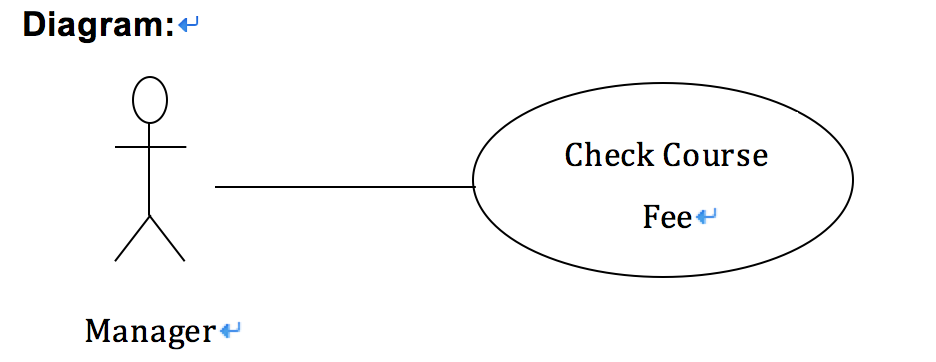
\includegraphics{216.PNG}
\end{figure}
\paragraph{}
\begin{flushleft}
\textbf{Brief Description }
\paragraph{}
The Administer logs in the WeChat Volunteering Website, check course fee and view courses.\\

\begin{flushleft}
\textbf{Initial Step-By-Step Description }
\paragraph{}
Before this use case can be initiated, the Manager has already logged in the WeChat Volunteering Website.

\begin{flushleft}
1.	The Manager chooses course. \\
2.	The System presents the list of courses information.  \\
3.	The Manager chooses a course.\\
4.	The System presents the details of the course and the list of Users enrolling in it. \\
5.	The Manager check the fee from the bank. \\
6.	The Manager presses confirm the payment if the fee is received from the volunteer. \\
7.	The System changes the state for the User to already paid. \\
Xref: Section 3.1.30, Check Course Fee
\end{flushleft}
\end{flushleft}
\end{flushleft}


%2.17
\newpage
\subsubsection{Use case:  View Courses }

\begin{figure}[!htb]
  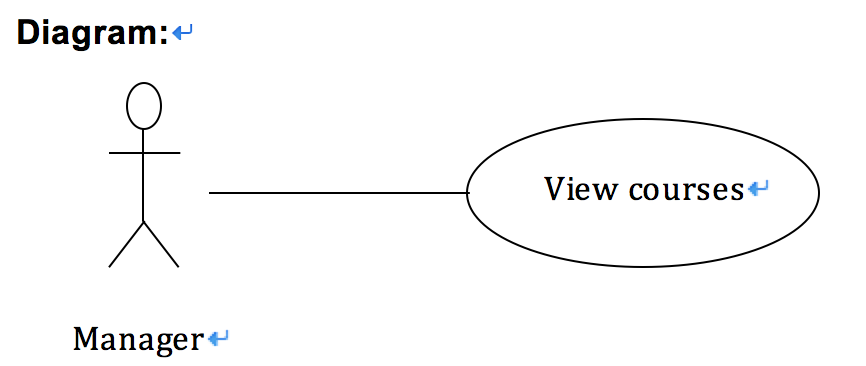
\includegraphics{217.PNG}
\end{figure}
\paragraph{}
\begin{flushleft}
\textbf{Brief Description }
\paragraph{}
The Manager logs in the WeChat Volunteering Website, view courses.\\

\begin{flushleft}
\textbf{Initial Step-By-Step Description }
\paragraph{}
Before this use case can be initiated, the Manager has already logged in the WeChat Volunteering Website.

\begin{flushleft}
1.	The Manager chooses course. \\
2.	The System presents the list of courses information. \\
3.	The Manager chooses a course. \\
4.	The System presents the details of the course and the list of Users enrolling in it to the Manager. \\
Xref: Section 3.1.31, View Courses
\end{flushleft}
\end{flushleft}
\end{flushleft}

%2.18
\newpage
\subsubsection{Use case:  View projects }

\begin{figure}[!htb]
  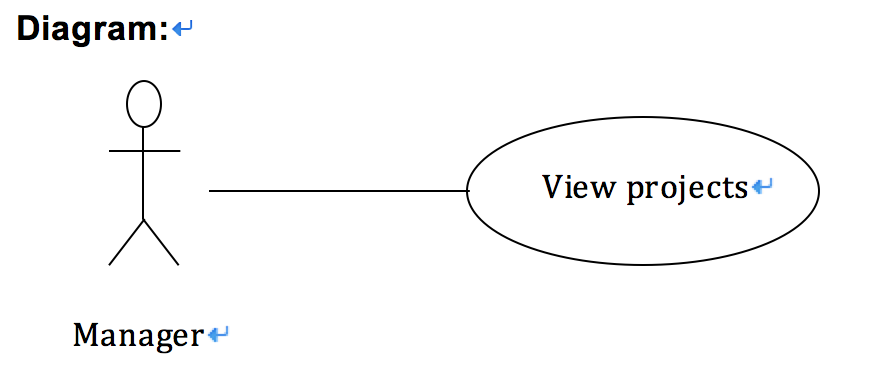
\includegraphics{218.PNG}
\end{figure}
\paragraph{}
\begin{flushleft}
\textbf{Brief Description }
\paragraph{}
The Manager logs in the WeChat Volunteering Website, view projects.\\

\begin{flushleft}
\textbf{Initial Step-By-Step Description }
\paragraph{}
Before this use case can be initiated, the Manager has already logged in the WeChat Volunteering Website.

\begin{flushleft}
1.	The Manager chooses social activities. \\
2.	The System presents the list of projects information. \\
3.	The Manager chooses a project. \\
4.	The System presents the details of the project and list of Users enrolling in it to the Manager.\\
Xref: Section 3.1.32, View projects
\end{flushleft}
\end{flushleft}
\end{flushleft}



\newpage
\section{Functional Requirements}
\subsection{ System Requirements}
\subsubsection{Check member manual}
\paragraph{}

\begin{tabular}{|c|l|}
\hline
Use Case Name & \makecell[c]{Check member manual} \\
\hline
XRef & Section 2.1.1, Check member manual \\
\hline
Trigger & The Volunteer has selected to check member manual.\\
\hline
\multirow{2}{*}{} 
Precondition & \makecell[l]{The Volunteer has registered, and accessed to "personal information" \\ page.} \\
\hline
\multirow{2}{*}{} 
Basic Path & \makecell[l]{1.The system presents the member manual. \\ 2. The Volunteer may return to "personal information" page anytime.} \\
\hline
\multirow{2}{*}{} 
Alternative Paths & \makecell[l]{None. }\\
\hline 
\multirow{2}{*}{} 
Postcondition & \makecell[l]{The member manual has been displayed.} \\
\hline
Exception Paths & The Volunteer may abandon the operation at any time. \\
\hline
\multirow{2}{*}{} 
Other & \makecell[l]{None.}\\
\hline
\end{tabular}

%3.12
\subsubsection{Check credit record}
\paragraph{}

\begin{tabular}{|c|l|}
\hline
Use Case Name & \makecell[c]{CCheck credit record} \\
\hline
XRef & Section 2.1.2, Check credit record\\
\hline
Trigger & The Volunteer has selected to check credit record.\\
\hline
\multirow{2}{*}{} 
Precondition & \makecell[l]{The Volunteer has registered, and accessed to "personal information" \\ page.} \\
\hline
\multirow{2}{*}{} 
Basic Path & \makecell[l]{1.The system shows the total number of score. \\
2.The Volunteer may request to see his each time record. \\
3.The system presents a list of the volunteer?s score record.} \\
\hline
\multirow{2}{*}{} 
Alternative Paths & \makecell[l]{None. }\\
\hline 
\multirow{2}{*}{} 
Postcondition & \makecell[l]{The requested information has been displayed.} \\
\hline
Exception Paths & The Volunteer may abandon the operation at any time. \\
\hline
\multirow{2}{*}{} 
Other & \makecell[l]{None.}\\
\hline
\end{tabular}


%3.13
\subsubsection{Check personal information}
\paragraph{}

\begin{tabular}{|c|l|}
\hline
Use Case Name & \makecell[c]{Check personal information} \\
\hline
XRef & Section 2.1.3, Check personal information \\
\hline
Trigger & TThe Volunteer has selected to check personal information.\\
\hline
\multirow{2}{*}{} 
Precondition & \makecell[l]{The Volunteer has registered, and accessed to "personal information" \\ page.} \\
\hline
\multirow{2}{*}{} 
Basic Path & \makecell[l]{1. The system shows volunteer personal information} \\
\hline
\multirow{2}{*}{} 
Alternative Paths & \makecell[l]{None. }\\
\hline 
\multirow{2}{*}{} 
Postcondition & \makecell[l]{The requested information has been displayed.} \\
\hline
Exception Paths & The Volunteer may abandon the operation at any time. \\
\hline
\multirow{2}{*}{} 
Other & \makecell[l]{None.}\\
\hline
\end{tabular}

%3.14
\subsubsection{Check activity record}
\paragraph{}

\begin{tabular}{|c|l|}
\hline
Use Case Name & \makecell[c]{Check member manual} \\
\hline
XRef & Section 2.1.4, Check activity record \\
\hline
Trigger & The Volunteer has registered, and accessed to `personal information` page.\\
\hline
\multirow{2}{*}{} 
Precondition & \makecell[l]{The Volunteer has registered, and accessed to "personal information" \\ page.} \\
\hline
\multirow{2}{*}{} 
Basic Path & \makecell[l]{1.The system shows the total number of activity that the volunteer has \\ participated. \\ 2.The Volunteer may request to see the full record about his activities. \\
3. The system presents a list of the volunteer`s activity record, and every \\ record links to its activity details.} \\
\hline
\multirow{2}{*}{} 
Alternative Paths & \makecell[l]{None. }\\
\hline 
\multirow{2}{*}{} 
Postcondition & \makecell[l]{The requested information has been displayed.} \\
\hline
Exception Paths & The Volunteer may abandon the operation at any time. \\
\hline
\multirow{2}{*}{} 
Other & \makecell[l]{None.}\\
\hline
\end{tabular}

%3.15
\subsubsection{Check submit application}
\paragraph{}

\begin{tabular}{|c|l|}
\hline
Use Case Name & \makecell[c]{Check submit application} \\
\hline
XRef & Section 2.1.5, Check submit application \\
\hline
Trigger & The Volunteer has selected to status request.\\
\hline
\multirow{2}{*}{} 
Precondition & \makecell[l]{The Volunteer has registered, and accessed to "personal information" \\ page.} \\
\hline
\multirow{2}{*}{} 
Basic Path & \makecell[l]{1.The system shows a text area and a "submit" button. \\
2.The Volunteer need to write down his application, and click "submit". \\
3.The system presents ?submit fail? if the volunteer credits is not enough, \\ or "submit succeed". \\
4.  If submit succeed, the system will show "Pending" \\ at previous ?Submit? button.} \\
\hline
\multirow{2}{*}{} 
Alternative Paths & \makecell[l]{None. }\\
\hline 
\multirow{2}{*}{} 
Postcondition & \makecell[l]{The application has been submitted.} \\
\hline
\multirow{3}{*}{} 
Exception Paths & \makecell[l]{1.	The Volunteer may abandon the operation at any time. \\
2. The Volunteer may not write down any word. \\
3. The Volunteer may leave before submitting. }\\
\hline
\multirow{2}{*}{} 
Other & \makecell[l]{None.}\\
\hline
\end{tabular}

%3.16
\subsubsection{Check study record }
\paragraph{}

\begin{tabular}{|c|l|}
\hline
Use Case Name & Check study record \\
\hline
XRef & Section 2.1.6, Check study record \\
\hline
Trigger & The Volunteer has selected to check study record.\\
\hline
\multirow{2}{*}{} 
Precondition & \makecell[l]{The Volunteer has registered, and accessed to "personal information" \\ page.} \\
\hline
\multirow{3}{*}{} 
Basic Path & \makecell[l]{
1.	The system shows the total number of study record that the volunteer \\ has participated. \\
2.	The Volunteer may request to see the whole record about his study. \\
3.	The system presents a list of the volunteer`s study record, and every\\ record links to its class details.} \\
\hline
\multirow{2}{*}{} 
Alternative Paths & \makecell[l]{None. }\\
\hline 
\multirow{2}{*}{} 
Postcondition & \makecell[l]{The requested information has been displayed.} \\
\hline
Exception Paths & The Volunteer may abandon the operation at any time. \\
\hline
\multirow{2}{*}{} 
Other & \makecell[l]{None.}\\
\hline
\end{tabular}

%3.17
\subsubsection{Attend projects}
\paragraph{}

\begin{tabular}{|c|l|}
\hline
Use Case Name & \makecell[c]{Attend projects} \\
\hline
XRef & Section 2.1.7, Attend projects \\
\hline
\multirow{2}{*}{} 
Trigger & \makecell[l]{Before this use case can be initiated, the User has already logged in the \\ WeChat Volunteering Website.}\\
\hline
\multirow{2}{*}{} 
Precondition & \makecell[l]{The User has accessed to the user`s homepage.} \\
\hline
\multirow{2}{*}{} 
Basic Path & \makecell[l]{
1.	The User chooses social activities. \\
2.	The System presents the list of projects information. \\
3.	The User chooses a project to attend. \\
4.	The System presents the details of the project. \\
5.	The User presses enroll button.  \\
6.	The System enrolls the volunteer in the database if the condition is\\ satisfied.} \\
\hline
\multirow{2}{*}{} 
Alternative Paths & \makecell[l]{In step 5, if the User chooses preview: \\
1. The system displays the previous page. }\\
\hline 
\multirow{2}{*}{} 
Postcondition & \makecell[l]{The User is added to the project in the database.} \\
\hline
Exception Paths &The User may abandon enrollment at any time. \\
\hline
\multirow{2}{*}{} 
Other & \makecell[l]{None.}\\
\hline
\end{tabular}

%3.18
\subsubsection{View projects}
\paragraph{}

\begin{tabular}{|c|l|}
\hline
Use Case Name & \makecell[c]{View projects} \\
\hline
XRef & Section 2.1.8, View projects \\
\hline
\multirow{2}{*}{} 
Trigger & \makecell[l]{Before this use case can be initiated, the User has already logged in the \\ WeChat Volunteering Website.}\\
\hline
\multirow{2}{*}{} 
Precondition & \makecell[l]{The User has accessed to the manager?s homepage.} \\
\hline
\multirow{2}{*}{} 
Basic Path & \makecell[l]{1.The User chooses social activities. \\
2.The System presents the list of projects information. \\
3.The User chooses a project. \\
4.The System presents the details of the project to the User.} \\
\hline
\multirow{3}{*}{} 
Alternative Paths & \makecell[l]{In step 3, if the User wants to see other parts: \\
1.	The User chooses preview. \\
2.	The system presents the previous page.
}\\
\hline 
\multirow{2}{*}{} 
Postcondition & \makecell[l]{The project? detailed information is presented.} \\
\hline
Exception Paths & The User may abandon viewing at any time. \\
\hline
\multirow{2}{*}{} 
Other & \makecell[l]{None.}\\
\hline
\end{tabular}

%3.19
\subsubsection{View Courses}
\paragraph{}

\begin{tabular}{|c|l|}
\hline
Use Case Name & \makecell[c]{View Courses} \\
\hline
XRef & Section 2.1.9, View Courses \\
\hline
\multirow{2}{*}{} 
Trigger & \makecell[l]{Before this use case can be initiated, the User has already logged in the \\ WeChat Volunteering Website.}\\
\hline
\multirow{2}{*}{} 
Precondition & \makecell[l]{The User has accessed to the manager?s homepage.} \\
\hline
\multirow{5}{*}{} 
Basic Path & \makecell[l]{
1.	The User chooses course. \\
2.	The System presents the list of courses information.  \\
3.	The User chooses a course. \\
4.	The System presents the details of the course to the User .
} \\
\hline
\multirow{3}{*}{} 
Alternative Paths & \makecell[l]{
In step 3, if the User wants to see other parts: \\
1.	The User chooses preview. \\
2.	The system presents the previous page.
 }\\
\hline 
\multirow{2}{*}{} 
Postcondition & \makecell[l]{The course? detailed information is presented.} \\
\hline
Exception Paths & The User  may abandon viewing at any time.\\
\hline
\multirow{2}{*}{} 
Other & \makecell[l]{None.}\\
\hline
\end{tabular}

%3.110
\subsubsection{Attend Coursel}
\paragraph{}

\begin{tabular}{|c|l|}
\hline
Use Case Name & \makecell[c]{Attend Course} \\
\hline
XRef & Section 2.1.10, Attend Course \\
\hline
\multirow{2}{*}{} 
Trigger & \makecell[l]{Before this use case can be initiated, the User has already logged in the \\ WeChat Volunteering Website.}\\
\hline
\multirow{2}{*}{} 
Precondition & \makecell[l]{The User has accessed to the user`s homepage.} \\
\hline
\multirow{2}{*}{} 
Basic Path & \makecell[l]{
1.	The User chooses course. \\
2.	The system presents s list of courses. \\
3.	The User chooses a course to enroll. \\
4.	The system presents the details of the course. \\
5.	The User presses enroll button. \\
6.	The system presents a box containing a bank account and a button \\already paid. \\
7.	The User pays the course fee to the account and presses the button \\already paid.} \\
\hline
\multirow{2}{*}{} 
Alternative Paths & \makecell[l]{In step 5, if the User chooses preview: \\
The system displays the previous page.}\\
\hline 
\multirow{2}{*}{} 
Postcondition & \makecell[l]{The User is added to the course in the database.
} \\
\hline
Exception Paths &The User may abandon enrollment at any time.\\
\hline
\multirow{2}{*}{} 
Other & \makecell[l]{None.}\\
\hline
\end{tabular}

%3.111
\subsubsection{Sign up}
\paragraph{}

\begin{tabular}{|c|l|}
\hline
Use Case Name & \makecell[c]{Sign up} \\
\hline
XRef & Section 2.1.11, Sign up\\
\hline
Trigger & The user selects a sign up link.\\
\hline
\multirow{2}{*}{} 
Precondition & \makecell[l]{The user needs to follow the Wechat public number with interest.} \\
\hline
\multirow{2}{*}{} 
Basic Path & \makecell[l]{
1.	The system presents an interface to receive the sign up information. \\
2.	The users try to complete all the information they need to fill. \\
3.	The users complete all the information, click the finish. \\
4.	The system records the information and exist the page. 
} \\
\hline
\multirow{2}{*}{} 
Alternative Paths & \makecell[l]{If the user`s entering information isn`t belong to the correct \\ format the system need to remind the user to complete it again.}\\
\hline 
\multirow{2}{*}{} 
Postcondition & \makecell[l]{The sign up is completed.} \\
\hline
Exception Paths & The attempt may be abandoned at any time. \\
\hline
\multirow{2}{*}{} 
Other & \makecell[l]{None.}\\
\hline
\end{tabular}

%3.112
\subsubsection{Log in}
\paragraph{}

\begin{tabular}{|c|l|}
\hline
Use Case Name & \makecell[c]{Log in} \\
\hline
XRef & Section 2.1.12, Log in \\
\hline
Trigger & The user selects a log in link.\\
\hline
\multirow{2}{*}{} 
Precondition & \makecell[l]{The user needs to sign up an account for logging in.} \\
\hline
\multirow{2}{*}{} 
Basic Path & \makecell[l]{
1.	The system presents an interface to receive the log in information. \\
2.	The users enter the account and password then submit. \\
3.	The system checks if the account and password is correct. \\
4.	The user successfully logs into the system or enter again.} \\
\hline
\multirow{2}{*}{} 
Alternative Paths & \makecell[l]{If the account of the user entering isn`t existed, \\ the system will hint the user to sign up first.}\\
\hline 
\multirow{2}{*}{} 
Postcondition & \makecell[l]{User log into the system successfully.} \\
\hline
Exception Paths &The attempt may be abandoned at any time.  \\
\hline
\multirow{2}{*}{} 
Other & \makecell[l]{None.}\\
\hline
\end{tabular}

%3.1.13
\subsubsection{Complete the personal information}
\paragraph{}

\begin{tabular}{|c|l|}
\hline
Use Case Name & \makecell[c]{Complete the personal information} \\
\hline
XRef & Section 2.1.13, Complete the personal information \\
\hline
Trigger & TThe user selects a sign up link.\\
\hline
\multirow{2}{*}{} 
Precondition & \makecell[l]{The user needs to start the sign up process.} \\
\hline
\multirow{5}{*}{} 
Basic Path & \makecell[l]{
1.	The system provides the name, telephone number, address, gender and \\birthday for user to filling up. \\
2.	The user complete each blank with the own information. \\
3.	The system check the correctness of the entering information. \\
4.	The user completes it or does it again with wrong format of the \\information.} \\
\hline
\multirow{2}{*}{} 
Alternative Paths & \makecell[l]{The user may forget to fill some of the information \\ so that the information process can`t be completed. }\\
\hline 
\multirow{2}{*}{} 
Postcondition & \makecell[l]{User completes the personal information successfully.} \\
\hline
Exception Paths & The attempt may be abandoned at any time.  \\
\hline
\multirow{2}{*}{} 
Other & \makecell[l]{None.}\\
\hline
\end{tabular}

%3.1.14
\subsubsection{Edit the information}
\paragraph{}

\begin{tabular}{|c|l|}
\hline
Use Case Name & \makecell[c]{Edit the information} \\
\hline
XRef & Section 2.1.14, Edit the information \\
\hline
Trigger & The user selects a edit link.\\
\hline
\multirow{2}{*}{} 
Precondition & \makecell[l]{The user needs to access to the system.} \\
\hline
\multirow{2}{*}{} 
Basic Path & \makecell[l]{
1.	The user want to edit the personal information. \\
2.	The system provide a page for user to edit the information which \\they want to. \\
3.	The user completes the edit process. \\
4.	The system stores the information to the database.} \\
\hline
\multirow{2}{*}{} 
Alternative Paths & \makecell[l]{If the entering information`s format by the user is wrong then the system \\ would remind that the user needs to enter the correct format information.  
 }\\
\hline 
\multirow{2}{*}{} 
Postcondition & \makecell[l]{User edits the information successfully.} \\
\hline
Exception Paths & If the edited information blank is empty then there will be an error. \\
\hline
\multirow{2}{*}{} 
Other & \makecell[l]{None.}\\
\hline
\end{tabular}


%3.1.15
\subsubsection{Initiate learning and growth}
\paragraph{}

\begin{tabular}{|c|l|}
\hline
Use Case Name & \makecell[c]{Initiate learning and growth} \\
\hline
XRef & Section 2.1.15, Initiate learning and growth \\
\hline
Trigger & The Manager assesses the Online Website and selects to add new lessons.\\
\hline
\multirow{2}{*}{} 
Precondition & \makecell[l]{The Manager has accessed the ?Add lesson? window.} \\
\hline
\multirow{8}{*}{} 
Basic Path & \makecell[l]{
1.	The Manager selects to `Leaning and Growth`. \\
2.	The system displays the previous lessons has been initiated by Manager. \\
3.	The Manager chooses `Add new` button. \\
4.	The system displays the details which have to be filled by Manager. \\
5.	The Manager fill in some details about this lesson. \\
6.	The Manager presses the `Publish` button. \\
7.	The system transfers the lesson information to the website and returns \\ the Manager to the main page of lesson } \\
\hline
\multirow{7}{*}{} 
Alternative Paths & \makecell[l]{In step 6, if the Manager press `Preview` button \\
7.The system displays the preview page. \\
8.The Manager presses `back`. \\
9.The system returns the manager to `Add new` page. \\
In step 8, if the Manager press `Publish` button \\
9.The system transfers the lesson information to the website and returns \\ the Manager to \\ the main page of lesson. }\\
\hline 
\multirow{2}{*}{} 
Postcondition & \makecell[l]{The new lesson is published to website and all of the users can see and \\ sign up.} \\
\hline
Exception Paths & The Manager may abandon the add at any time. \\
\hline
\multirow{6}{*}{} 
Other & \makecell[l]{The details about new lesson include main picture, theme, start time, \\end time, specific address, numbers, integral, status, reward, cost, remittance \\ information, discount, activity details. \\
The picture part: The Manager have to upload one representative photo or \\short video. \\
The discount part: fill in the percent \\
The remittance information part: The Manager can choose one of account \\which we have.}\\
\hline
\end{tabular}

%3.1.16
\subsubsection{Edit learning and growth}
\paragraph{}

\begin{tabular}{|c|l|}
\hline
Use Case Name & \makecell[c]{Edit learning and growth} \\
\hline
XRef & Section 2.1.16, Edit learning and growth\\
\hline
Trigger & The Manager assesses the Online Website and selects to edit lessons.\\
\hline
\multirow{2}{*}{} 
Precondition & \makecell[l]{The Manager has accessed the `Edit` page.} \\
\hline
\multirow{7}{*}{} 
Basic Path & \makecell[l]{
1.	The Manager selects to ``Learning and Growth``. \\
2.	The system displays the previous lessons has been initiated by Manager. \\
3.	The Manager chooses one of the initiated lessons and press `Edit` button. \\
4.	The system displays the edit page. \\
5.	The Manager edits some details about this lesson and presses the \\`Publish` button. \\
6.	The system transfers the lesson information to the website and returns\\ the Manager to the main page of lesson.} \\
\hline
\multirow{7}{*}{} 
Alternative Paths & \makecell[l]{In step 6, if the Manager press `Preview` button \\
7.The system displays the preview page. \\
8.The Manager press `back`. \\
9.The system returns the manager to `Edit` page. \\
In step 8, if the Manager press `Publish` button \\
9.The system transfers the lesson information to the website and returns \\the Manager to the main page of lesson.}\\
\hline 
\multirow{2}{*}{} 
Postcondition & \makecell[l]{The edited lesson is published to website and all of the users can see and \\ sign up.} \\
\hline
Exception Paths & The Manager may abandon the edit at any time. \\
\hline
\multirow{3}{*}{} 
Other & \makecell[l]{The details about new lesson include main picture, theme, start time, \\ end time, specific address, numbers, integral, status, reward, cost, \\remittance information, discount, activity details.}\\
\hline
\end{tabular}

%3.1.17
\subsubsection{Identity authentication}
\paragraph{}

\begin{tabular}{|c|l|}
\hline
Use Case Name & \makecell[c]{Identity authentication} \\
\hline
XRef & Section 2.1.17, Identity authentication \\
\hline
Trigger & The Manager has accessed the web system and in the Identity audit page.\\
\hline
\multirow{2}{*}{} 
Precondition & \makecell[l]{There are some applications in the list.} \\
\hline
\multirow{2}{*}{} 
Basic Path & \makecell[l]{
1.	The Manager selects to `Identity authentication`. \\
2.	The system displays the application list with applier names, identities, \\and apply time. \\
3.	The Manager can choose one of the applications. \\
4.	The system displays the detailed personal information. \\
5.	The Manager will choose `Agree` or `Disagree` based on the personal \\ information. \\
6.	The system will put this application into `Already Audited` page.} \\
\hline
\multirow{6}{*}{} 
Alternative Paths & \makecell[l]{In step 5, if the Manager chooses `Disagree` and give reasons. \\
6.The system jumps to a new page which displays the grids for Manager to\\ fill in some reasons why the application does not pass. \\
7.The Manager fills in the reasons and press `Send`. \\
8.The system sends failed message and reasons to applier and puts this\\ application into `Already Audited` page .}\\
\hline 
\multirow{2}{*}{} 
Postcondition & \makecell[l]{The applications are authenticated however successful or failed.} \\
\hline
Exception Paths & The Manager may abandon the authentication or fills in reasons at any time. \\
\hline
\multirow{2}{*}{} 
Other & \makecell[l]{When Manager abandon the authentication halfway, this application will be \\ sent back to the list whose applications are to be authenticated.}\\
\hline
\end{tabular}


%3.1.18
\subsubsection{Add activity records}
\paragraph{}

\begin{tabular}{|c|l|}
\hline
Use Case Name & \makecell[c]{Add activity records} \\
\hline
XRef & Section 2.1.18, Add activity records \\
\hline
Trigger & The Manager assesses the Online Website and in the Add activity records\\ page\\
\hline
\multirow{2}{*}{} 
Precondition & \makecell[l]{The Web is displayed with grids for adding records which activity has \\ finished not very soon.} \\
\hline
\multirow{2}{*}{} 
Basic Path & \makecell[l]{
1.	The Manager selects to `Activity records`. \\
2.	The system displays the previous activity records. \\
3.	The Manager chooses `Add new` button. \\
4.	The system displays some details which Manager have to fill in. \\
5.	The Manager fills in the details and publish the records. \\
6.	The system transfers records to the website and returns Manager to \\the main page.} \\
\hline
\multirow{2}{*}{} 
Alternative Paths & \makecell[l]{In step 3, if Manager chooses `Edit` button. \\
4.	The system displays records which are not finished. \\
5.	The Manager chooses one of them to edit. \\
6.	The system displays the record page which have to be filled in by \\Manager. \\
In step 5, if the abandon editing records and chooses `Save` button. \\
6.The system save the changed which have been made.}\\
\hline 
\multirow{2}{*}{} 
Postcondition & \makecell[l]{The new records are finished and transferred to the website which can\\ be read by every user.} \\
\hline
Exception Paths & The Manager may abandon the editing at any time. \\
\hline
\multirow{2}{*}{} 
Other & \makecell[l]{The Manager abandon the editing of the records, the system should \\save changes which have been made.}\\
\hline
\end{tabular}


%3.1.19
\subsubsection{View users list}
\paragraph{}

\begin{tabular}{|c|l|}
\hline
Use Case Name & \makecell[c]{View users list} \\
\hline
XRef & Section 2.1.15, View users list \\
\hline
Trigger & The Manager assesses the Online Website\\
\hline
\multirow{2}{*}{} 
Precondition & \makecell[l]{None.} \\
\hline
\multirow{2}{*}{} 
Basic Path & \makecell[l]{
1.	The Manager selects to `View users`. \\
2.	The system displays the users list including users? basic information.} \\
\hline
\multirow{2}{*}{} 
Alternative Paths & \makecell[l]{None. }\\
\hline 
\multirow{2}{*}{} 
Postcondition & \makecell[l]{The users list has been displayed. .} \\
\hline
Exception Paths & The Manager may abandon the operation at any time. \\
\hline
\multirow{2}{*}{} 
Other & \makecell[l]{None.}\\
\hline
\end{tabular}

%3.1.20
\subsubsection{Search users}
\paragraph{}

\begin{tabular}{|c|l|}
\hline
Use Case Name & \makecell[c]{Search users} \\
\hline
XRef & Section 2.1.20, Search users \\
\hline
Trigger & The Manager assesses the Online Website and in the search page.\\
\hline
\multirow{2}{*}{} 
Precondition & \makecell[l]{The Web is displayed with grids for searching} \\
\hline
\multirow{2}{*}{} 
Basic Path & \makecell[l]{
1.	The Manager selects to `Search users`. \\
2.	The system displays the page of the search. \\
3.	The Manager type user`s phone number that want to search. \\
4.	The system displays the list of phone number which is searched.} \\
\hline
\multirow{2}{*}{} 
Alternative Paths & \makecell[l]{In step 3, if the Manager selects to search by name . \\
1.	The system displays the list of name which is searched. }\\
\hline 
\multirow{2}{*}{} 
Postcondition & \makecell[l]{The requested user`s information has been displayed.} \\
\hline
Exception Paths & The Manager may abandon the search at any time. \\
\hline
\multirow{2}{*}{} 
Other & \makecell[l]{None.}\\
\hline
\end{tabular}

%3.1.21
\subsubsection{View users` details}
\paragraph{}

\begin{tabular}{|c|l|}
\hline
Use Case Name & \makecell[c]{View users` details} \\
\hline
XRef & Section 2.1.21, View users` details \\
\hline
Trigger & The Manager assesses the Online Website.\\
\hline
\multirow{2}{*}{} 
Precondition & \makecell[l]{The Web is displayed with all of the users signed up.} \\
\hline
\multirow{2}{*}{} 
Basic Path & \makecell[l]{
1.	The Manager selects to `View users`. \\
2.	The system displays the users list. \\
3.	The Manager can choose one specific user. \\
4.	The system displays the detailed personal information of the user.} \\
\hline
\multirow{2}{*}{} 
Alternative Paths & \makecell[l]{In step 3, if the Manager want to find goal user immediately. \\
4.The Manager can use search function to input phone number or user \\name to search specific user. \\
5.	The system displays the list of user which is searched. \\
6.	The Manager chooses one who is wanted. \\
7.	The system displays the detailed information about the user who is \\searched. }\\
\hline 
\multirow{2}{*}{} 
Postcondition & \makecell[l]{The requested detailed information has been displayed. } \\
\hline
Exception Paths & The Manager may abandon the operation at any time. \\
\hline
\multirow{2}{*}{} 
Other & \makecell[l]{When the Manager checked one of the user`s information then, \\ Manager can choose `back` to the users list page to check other users`\\ detailed information. \\
The detailed information include: Name, Gender, Birthday, Phone number,\\ Address, Identity, activity numbers, course numbers and Integral.}\\
\hline
\end{tabular}

%3.1.22
\subsubsection{View users` details}
\paragraph{}

\begin{tabular}{|c|l|}
\hline
Use Case Name & \makecell[c]{View users` details} \\
\hline
XRef & Section 2.1.22, View users` details \\
\hline
Trigger &The Manager assesses the Online Website and in the `View activities` page.\\
\hline
\multirow{2}{*}{} 
Precondition & \makecell[l]{There is activity which is not held.} \\
\hline
\multirow{2}{*}{} 
Basic Path & \makecell[l]{
1.	The Manager selects to `View activities`. \\
2.	The system displays the public-spirited activities which are not be held. \\
3.	The Manager can choose `Generate QR code` button.  \\
4.	The system generates the QR code and displays it on the screen.} \\
\hline
\multirow{2}{*}{} 
Alternative Paths & \makecell[l]{None. }\\
\hline 
\multirow{2}{*}{} 
Postcondition & \makecell[l]{The QR code has been displayed.} \\
\hline
Exception Paths & The Manager may generate the QR code many times. \\
\hline
\multirow{2}{*}{} 
Other & \makecell[l]{No matter how many times the Manager generate the QR code, \\ the code can be scanned as attendance sheet for this activity.}\\
\hline
\end{tabular}

%3.1.23
\subsubsection{Modify user credit}
\paragraph{}

\begin{tabular}{|c|l|}
\hline
Use Case Name & \makecell[c]{Modify user credit} \\
\hline
XRef & Section 2.1.23, Modify user credit\\
\hline
\multirow{2}{*}{} 
Trigger & \makecell[l]{ Before this use case can be initiated, the Manager has \\already accessed the manager interface and select Credit Management section.}\\
\hline
\multirow{2}{*}{} 
Precondition & \makecell[l]{The System displays an input area for searching} \\
\hline
\multirow{2}{*}{} 
Basic Path & \makecell[l]{
1.	The manager types in user?s phone number. \\
2.	The system displays the user?s name. \\
3.	The manager types in number of credits want to modify. \\
4.	The manager chooses the reason of modification among charity activity, \\courses and other. \\
5.	The manager confirms modification. \\
6.	The system modify user credit record} \\
\hline
\multirow{2}{*}{} 
Alternative Paths & \makecell[l]{In step 1, if the manager inputs a invalid number: \\
1.	the system displays an alert saying user doesn`t exit. \\
2.	The Manager clicks ok and back to initial state again. }\\
\hline 
\multirow{2}{*}{} 
Postcondition & \makecell[l]{The user`s credit changes in the database.} \\
\hline
Exception Paths & The Reader may abandon modification at any time. \\
\hline
\multirow{2}{*}{} 
Other & \makecell[l]{None.}\\
\hline
\end{tabular}

%3.1.24
\subsubsection{View users` credit}
\paragraph{}

\begin{tabular}{|c|l|}
\hline
Use Case Name & \makecell[c]{View users` credit} \\
\hline
XRef & Section 2.1.24, View users` credit \\
\hline
Trigger & The Editor has selected to users` credit management section.\\
\hline
\multirow{2}{*}{} 
Precondition & \makecell[l]{The Manager has already accessed the manager interface.} \\
\hline
\multirow{2}{*}{} 
Basic Path & \makecell[l]{
1.	The Manager chooses the credit management button.  \\
2.	The System shows the list of all credit modification record, sorted\\ by time. \\
3.	The Manager clicks one user`s name. \\
4.	The System displays this user`s credit modification records.} \\
\hline
\multirow{2}{*}{} 
Alternative Paths & \makecell[l]{None. }\\
\hline 
\multirow{2}{*}{} 
Postcondition & \makecell[l]{The requested information has been displayed.} \\
\hline
Exception Paths & The Editor may abandon the operation at any time. \\
\hline
\multirow{2}{*}{} 
Other & \makecell[l]{
1.	The record consists user name, phone number, modification date,\\ reason and number of credit. \\
2.	The list is sorted by date}\\
\hline
\end{tabular}


%3.1.25
\subsubsection{Add Charge Information}
\paragraph{}

\begin{tabular}{|c|l|}
\hline
Use Case Name & \makecell[c]{Add Charge Information} \\
\hline
XRef & Section 2.2.11, Add Charge Information \\ 
\hline
Trigger & The Manager selects to add a new charge information to the database.\\
\hline
\multirow{2}{*}{} 
Precondition & \makecell[l]{The Manager has already accessed the manager interface.} \\
\hline
\multirow{7}{*}{} 
Basic Path & \makecell[l]{
1.	The Manager chooses Finance Management button. \\
2.	The System display current accounts information. \\
3.	The Manager clicks New Account button. \\
4.	The System prompts Manager types in Name, Bank Name, \\and Account number. \\ 
5.	The Manager types in information. \\
6.	The Manager clicks Save button. \\
7.	The new account information saved in the system} \\
\hline
\multirow{2}{*}{} 
Alternative Paths & \makecell[l]{If in step 6, either field is blank, the Manager is instructed to \\ add an entry. No validation for correctness is made.
 }\\
\hline 
\multirow{2}{*}{} 
Postcondition & \makecell[l]{The New account information has been added to the database. } \\
\hline
Exception Paths & The Manager may abandon the operation at any time. \\
\hline
\multirow{2}{*}{} 
Other & \makecell[l]{The charge information includes account owner name, bank name \\and card number.}\\
\hline
\end{tabular}


%3.1.26
\subsubsection{Update Charge Information}
\paragraph{}

\begin{tabular}{|c|l|}
\hline
Use Case Name & \makecell[c]{Update Charge Information} \\
\hline
XRef & Section 2.2.12, Update Charge Information \\
\hline
Trigger & The Manager selects to edit a charge information in the database.\\
\hline
\multirow{2}{*}{} 
Precondition & \makecell[l]{The Manager has already accessed the manager interface.} \\
\hline
\multirow{2}{*}{} 
Basic Path & \makecell[l]{
1.	The Manager chooses Finance Management button. \\
2.	The System display current accounts information. \\
3.	The Manager clicks Edit button of one current account. \\
4.	The System enable Manager modifies Name, Bank Name, \\and Account number. \\
5.	The Manager types in information. \\
6.	The Manager clicks Save button. \\
7.	The modified account information saved in the system} \\
\hline
\multirow{2}{*}{} 
Alternative Paths & \makecell[l]{If in step 6, either field is blank, the Manager is instructed to \\ add an entry. No validation for correctness is made. }\\
\hline 
\multirow{2}{*}{} 
Postcondition & \makecell[l]{TThe New account information has been added to the database.} \\
\hline
Exception Paths & The Manager may abandon the operation at any time. \\
\hline
\multirow{2}{*}{} 
Other & \makecell[l]{The charge information includes account owner name, bank name \\and card number.}\\
\hline
\end{tabular}

%3.1.27
\subsubsection{Edit Discount Strategy}
\paragraph{}

\begin{tabular}{|c|l|}
\hline
Use Case Name & \makecell[c]{Edit Discount Strategy} \\
\hline
XRef & Section 2.2.13, Edit Discount Strategy \\
\hline
Trigger & The Editor selects to edit discount strategy.\\
\hline
\multirow{2}{*}{} 
Precondition & \makecell[l]{The Manager has already accessed the manager interface and \\ enter Discount Management section.} \\
\hline
\multirow{7}{*}{} 
Basic Path & \makecell[l]{
1.	The Manager chooses Discount Management button. \\
2.	The System displays current discount information with five different \\discount number for users \\ with different number of credits, before the first initialization, all numbers \\are zero.
3.	The Manager clicks edit button. \\
4.	The System enable Manager modify five numbers(percentage).\\
5.	The Manager modifies five discount numbers and clicks Save button. \\
6.	The system verifies the information and returns the Manager to Discount\\ Management page} \\
\hline
\multirow{2}{*}{} 
Alternative Paths & \makecell[l]{In step 5, system verifies if all number are valid, it not, system notifies \\Manager to modify it again. }\\
\hline 
\multirow{2}{*}{} 
Postcondition & \makecell[l]{The Discount Strategy has been modified to the database.} \\
\hline
Exception Paths & The Editor may abandon the operation at any time. \\
\hline
\multirow{2}{*}{} 
Other & \makecell[l]{The discount strategy is divided into five ranges, presented in percentage. \\
The discount strategy is initialized to 0 for all 5 groups\\
The groups are divided based on user credit. E.g. 0-100; 100-200; 200-300; \\300-400; \\
The number manager input shall within the range of 0-99(\%) }\\
\hline
\end{tabular}


%3.1.28
\subsubsection{Initial projects}
\paragraph{}

\begin{tabular}{|c|l|}
\hline
Use Case Name & \makecell[c]{Initial projects} \\
\hline
XRef & Section 2.2.14, Initial projects\\
\hline
\multirow{2}{*}{}
Trigger & \makecell[l]{Before this use case can be initiated, the Manager has already logged in\\ the WeChat Volunteering Website.}\\
\hline
\multirow{2}{*}{} 
Precondition & \makecell[l]{The Manager has accessed to the manager?s homepage.} \\
\hline
\multirow{14}{*}{} 
Basic Path & \makecell[l]{
1.	The Manager chooses social activities. \\
2.	The system presents the list of projects that have finished. \\
3.	The Manager presses add project record. \\
4.	The system shows a new page with empty project information to\\ be completed. \\
5.	The Manager complete the subject, start time, end time, detailed\\ address of the project,  the number of volunteers limited, score and\\ identity needed, as well as award. \\
6.	The Manager presses the text area for describing project details. \\
7.	The system presents an input box for typing to the Manager. \\
8.	The Manager presses finish to submit project details including photos\\ and videos. \\
9.	The system returns to the previous page. \\
10.	The Manager presses preview button. \\
11.	The system shows the appearance of the project after submitted. \\
12.	The Manager presses release button. \\
13.	The system releases the project so that volunteers can take part in.} \\
\hline
\multirow{2}{*}{} 
Alternative Paths & \makecell[l]{In step 5, if the manager`s input is empty: \\
1.	the system displays an error message. \\
2.	The Manager clicks ok and back to initial state again.}\\
\hline 
\multirow{2}{*}{} 
Postcondition & \makecell[l]{The new project is released in the website and all users can see and sign up.} \\
\hline
Exception Paths & The Manager may abandon addition at any time. \\
\hline
\multirow{2}{*}{} 
Other & \makecell[l]{None.}\\
\hline
\end{tabular}

%3.1.29
\subsubsection{Edit projects}
\paragraph{}

\begin{tabular}{|c|l|}
\hline
Use Case Name & \makecell[c]{Edit projects} \\
\hline
XRef & Section 2.2.15, Edit projects\\
\hline
\multirow{2}{*}{} 
Trigger & \makecell[l]{Before this use case can be initiated, the Manager has already logged in\\ the WeChat Volunteering Website.}\\
\hline
\multirow{2}{*}{} 
Precondition & \makecell[l]{The Manager has accessed to the manager`s homepage.} \\
\hline
\multirow{12}{*}{} 
Basic Path & \makecell[l]{
1.	The Manager chooses social activities. \\
2.	The system presents the list of projects. \\
3.	The Manager chooses not started. \\
4.	The system presents the list of projects that have not started yet. \\ 
5.	The Manager presses edit. \\
6.	The system presents a new page with the details of the project that can \\be edited. \\
7.	The Manager edits the details he/her want to change and remains others \\the same as before. \\
8.	The Manager presses preview. \\
9.	The system the appearance of the project after submitted. \\
10.	The Manager presses release button. \\
11.	The system releases the edited project.
} \\
\hline
\multirow{2}{*}{} 
Alternative Paths & \makecell[l]{In step 6, if the manager`s input is empty:\\
1.	the system displays an error message.\\
2.	The Manager clicks ok and back to initial state again. }\\
\hline 
\multirow{2}{*}{} 
Postcondition & \makecell[l]{The project`s information is changed and released in the website, that all \\ users can see and sign up.} \\
\hline
Exception Paths & The Manager may abandon edition at any time. \\
\hline
\multirow{2}{*}{} 
Other & \makecell[l]{None.}\\
\hline
\end{tabular}

%3.1.30
\subsubsection{Check Course Fee}
\paragraph{}
\begin{tabular}{|c|l|}
\hline
Use Case Name & \makecell[c]{Check Course Fee} \\
\hline
XRef & Section 2.2.16, Check Course Fee \\
\hline
\multirow{2}{*}{} 
Trigger &  \makecell[l]{Before this use case can be initiated, the Manager has already logged in\\ the WeChat Volunteering Website.}\\
\hline
\multirow{2}{*}{} 
Precondition & \makecell[l]{The Manager has accessed to the manager`s homepage.} \\
\hline
\multirow{7}{*}{} 
Basic Path & \makecell[l]{
1.	The Manager chooses course. \\
2.	The System presents the list of courses information.  \\
3.	The Manager chooses a course. \\
4.	The System presents the details of the course and the list of users \\enrolling in it. \\
5.	The Manager checks the fee from the bank. \\
6.	The Manager presses confirm the payment if the fee is received from\\ the user. \\
7.	The System changes the state for the user to already paid.
} \\
\hline
\multirow{3}{*}{} 
Alternative Paths & \makecell[l]{In step 6, if the manager receives no money:\\
1.	The Manager clicks preview. \\
2.	The system presents the previous page. }\\
\hline 
\multirow{2}{*}{} 
Postcondition & \makecell[l]{The condition of the fee is changed in both Manager and User page. }\\
\hline
Exception Paths & The Manager may abandon change at any time. \\
\hline
\multirow{2}{*}{} 
Other & \makecell[l]{None.}\\
\hline
\end{tabular}

%3.1.31
\subsubsection{View Courses}
\paragraph{}

\begin{tabular}{|c|l|}
\hline
Use Case Name & \makecell[c]{View Courses} \\
\hline
XRef & Section 2.2.17, View Courses \\
\hline
\multirow{2}{*}{} 
Trigger &  \makecell[l]{Before this use case can be initiated, the Manager has already logged in\\ the WeChat Volunteering Website.}\\
\hline
\multirow{2}{*}{} 
Precondition & \makecell[l]{The Manager has accessed to the manager`s homepage.} \\
\hline
\multirow{2}{*}{} 
Basic Path & \makecell[l]{
1.	The Manager chooses course. \\
2.	The System presents the list of courses information.  \\
3.	The Manager chooses a course. \\
The System presents the details of the course and the list of volunteers \\enrolling in it to the Manager.} \\
\hline
\multirow{2}{*}{} 
Alternative Paths & \makecell[l]{In step 3, if the Manager wants to see other parts:\\
1.	The Manager chooses preview. \\
2.	The system presents the previous page. }\\
\hline 
\multirow{2}{*}{} 
Postcondition & \makecell[l]{The course`s detailed information is presented.} \\
\hline
Exception Paths & The Manager may abandon viewing at any time. \\
\hline
\multirow{2}{*}{} 
Other & \makecell[l]{None.}\\
\hline
\end{tabular}

%3.1.32
\subsubsection{View projects}
\paragraph{}

\begin{tabular}{|c|l|}
\hline
Use Case Name & \makecell[c]{View projectsl} \\
\hline
XRef & Section 2.2.18, View projects \\
\hline
\multirow{2}{*}{} 
Trigger & \makecell[l]{Before this use case can be initiated, the Manager has already logged in\\ the WeChat Volunteering Website.}\\
\hline
\multirow{2}{*}{} 
Precondition & \makecell[l]{The Manager has accessed to the manager`s homepage.} \\
\hline
\multirow{2}{*}{} 
Basic Path & \makecell[l]{
1.	The Manager chooses social activities. \\
2.	The System presents the list of projects information. \\
3.	The Manager chooses a project.  \\
4.	The System presents the details of the project and the list of users\\ enrolling in it to the Manager.} \\
\hline
\multirow{2}{*}{} 
Alternative Paths & \makecell[l]{In step 3, if the Manager wants to see other parts: \\
1.	The Manager chooses preview. \\
2.	The system presents the previous page. }\\
\hline 
\multirow{2}{*}{} 
Postcondition & \makecell[l]{The project`s detailed information is presented.} \\
\hline
Exception Paths & The Manager may abandon viewing at any time. \\
\hline
\multirow{2}{*}{} 
Other & \makecell[l]{None.}\\
\hline
\end{tabular}
\\\\\\\\\\\\\\\\\\\\\\\\\\\\\\\\\\\\\\\\\\
%4
\section{Database}
\subsection{ER Diagram}
\begin{figure}[!htb]
  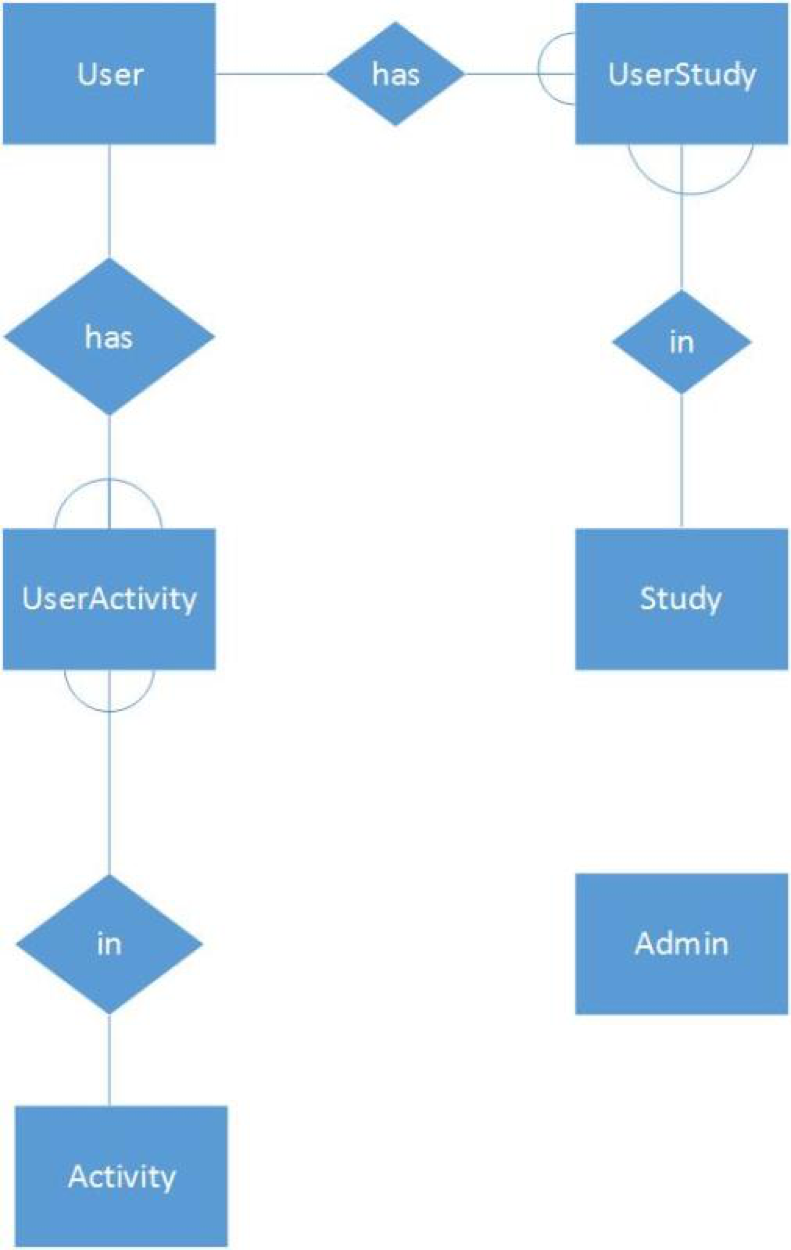
\includegraphics{0.PNG}
\end{figure}


\newpage
\subsection{Database}
%4.2.1
\newpage
\subsubsection{User}
\paragraph{}
\begin{tabular}{|c|c|l|c|}
\hline
Data Iterm & Type & Description & Comment \\
\hline
ID & Integer & ID of the normal user & Automatic increment\\
\hline
User Account & Text & The account of the normal & \\
\hline
\multirow{12}{*}{} 
User Password & Text &\makecell[l]{ The password of the corresponding\\ account.}&\\
\hline
Name & Text & Name of the normal user& \\
\hline
\multirow{12}{*}{} 
Telephone number & \makecell[l]{String of \\number} &\makecell[l]{The telephone number of the \\normal user}&\\
\hline 
Address & Text & The address of the normal user&\\
\hline
Exception Paths & Text & The address of the normal user &\\
\hline
Birthday & Text & The address of the normal user&\\
\hline
Gender & Text & Male or female &\\
\hline
\multirow{12}{*}{} 
Gredit & Integer &  \makecell[l]{The credit of a user that represent the \\different status} &\\
\hline 
\multirow{12}{*}{} 
Status & Integer &  \makecell[l]{There are different kinds of status for \\the user depend their point.}&\\
\hline
Register date & Date & The date of the user?s registration &\\
\hline
Activity number & Integer & \makecell[l]{The activity number which the user \\takes part in.} &\\
\hline
Study number & Integer & \makecell[l]{The study number which the user \\takes part in.}&\\
\hline
\end{tabular}

%4.2.2
\subsubsection{UserStudy}
\paragraph{}
\begin{tabular}{|c|c|l|c|}
\hline
Data Iterm & Type & Description & Comment \\
\hline
UserID & Integer & ID of the training which the user took part in&\\
\hline
StudyID & Integer & The ID number of the training which the user took part in &\\ 
\hline
\end{tabular}
%4.2.3
\subsubsection{Study}
\paragraph{}
\begin{tabular}{|c|c|l|c|}
\hline
Data Iterm & Type & Description & Comment \\
\hline
ID & Integer & ID of study & Automatic increment\\
\hline
Topic & Text & The theme of the study& \\
\hline
Begin time & Date & The start time of the study& \\
\hline
End time & Date & The end time of the study &\\
\hline
\multirow{12}{*}{} 
Number & Integer & \makecell[l]{The number that be allowed \\to apply for the study}&\\
\hline 
\multirow{12}{*}{} 
Registered number & Integer & \makecell[l]{The number that have registered \\for the study }& \\
\hline
Expenditure & Integer & The cost that apply for the study& \\
\hline
LimitStatus & INT & Level of volunteer &\makecell[l]{ Only this level or upper \\level volunteer can attend }\\
\hline
\multirow{12}{*}{} 
requireCredit & INT & \makecell[l]{Only have specific credit can attend\\ the activity}& \\
\hline
Detail & Text & \makecell[l]{The specific information about\\ the study} &\\
\hline 
\end{tabular}

%4.2.4
\subsubsection{Activity Data Entity}
\paragraph{}
\begin{tabular}{|c|c|l|c|}
\hline
Data Iterm & Type & Description & Comment \\
\hline
ActivityName & VARCHAR & Name of activity&\\
\hline
ActivityID & INT & ID number of the activity & Used as primary key \\
\hline
StartTime &
VARCHAR &
Activity start time&
 \\
\hline
EndTime &
VARCHAR &
Activity end time&
 \\
\hline
Address &
VARCHAR &
Location of activity&
\\
\hline 
LimitNum &
INT &
Limitation of number of Volunteer&
\\
\hline
CurNum &
INT &
Current number of volunteer &\\
\hline
\multirow{12}{*}{} 
LimitStatus &
INT &
Level of volunteer &
\makecell[l]{Only this level or upper \\level volunteer can attend} \\
\hline
\multirow{12}{*}{} 
requireCredit &
INT &
\makecell[l]{Only have specific credit\\ can attend the activity} &\\
\hline
Details &
VARCHAR &
Activity details &\\
\hline
\end{tabular}

%4.2.5
\subsubsection{User-activity Data Entity}
\paragraph{}
\begin{tabular}{|c|c|l|c|}
\hline
Data Iterm & Type & Description & Comment \\
\hline
activityID &
VARCHAR &
ID of activity &\\
\hline
userID &
VARCHAR  &
ID of user &
Used as primary key \\
\hline
attend &
Boolean &
Whether user attend the activity& \\
\hline
\end{tabular}

%4.2.6
\subsubsection{Application Data Entity}
\paragraph{}
\begin{tabular}{|c|c|l|c|}
\hline
Data Iterm & Type & Description & Comment \\
\hline
userName &
VARCHAR &
Name of volunteer& \\
\hline
userID &
INT &
ID number of volunteer &
Used as primary key \\
\hline
Statement &
VARCHAR &
Volunteer?s application &\\
\hline
\end{tabular}


%4.2.7
\subsubsection{Admin Data Entity}
\paragraph{}
\begin{tabular}{|c|c|l|c|}
\hline
Data Iterm & Type & Description & Comment \\
\hline
adminName &
VARCHAR &
Name of admin &\\
\hline
adminID &
INT &
ID number of admin &
Used as primary key \\
\hline
adminPW &
VARCHAR &
Admin?s password &\\
\hline
\end{tabular}


 
 \end{document}